%%%%%%%%%%%%%%%%%%%%%%%%%%%%%%%%%%%%%%%%%
% The Legrand Orange Book
% LaTeX Template
% Version 2.1.1 (14/2/16)
%
% This template has been downloaded from:
% http://www.LaTeXTemplates.com
%
% Original author:
% Mathias Legrand (legrand.mathias@gmail.com) with modifications by:
% Vel (vel@latextemplates.com)
%
% License:
% CC BY-NC-SA 3.0 (http://creativecommons.org/licenses/by-nc-sa/3.0/)
%
% Compiling this template:
% This template uses biber for its bibliography and makeindex for its index.
% When you first open the template, compile it from the command line with the 
% commands below to make sure your LaTeX distribution is configured correctly:
%
% 1) pdflatex main
% 2) makeindex main.idx -s StyleInd.ist
% 3) biber main
% 4) pdflatex main x 2
%
% After this, when you wish to update the bibliography/index use the appropriate
% command above and make sure to compile with pdflatex several times 
% afterwards to propagate your changes to the document.
%
% This template also uses a number of packages which may need to be
% updated to the newest versions for the template to compile. It is strongly
% recommended you update your LaTeX distribution if you have any
% compilation errors.
%
% Important note:
% Chapter heading images should have a 2:1 width:height ratio,
% e.g. 920px width and 460px height.
%
%%%%%%%%%%%%%%%%%%%%%%%%%%%%%%%%%%%%%%%%%

%----------------------------------------------------------------------------------------
%	PACKAGES AND OTHER DOCUMENT CONFIGURATIONS
%----------------------------------------------------------------------------------------

\documentclass[11pt,fleqn]{book} % Default font size and left-justified equations

\usepackage[toc,page]{appendix}
%----------------------------------------------------------------------------------------

%%%%%%%%%%%%%%%%%%%%%%%%%%%%%%%%%%%%%%%%%
% The Legrand Orange Book
% Structural Definitions File
% Version 2.0 (9/2/15)
%
% Original author:
% Mathias Legrand (legrand.mathias@gmail.com) with modifications by:
% Vel (vel@latextemplates.com)
% 
% This file has been downloaded from:
% http://www.LaTeXTemplates.com
%
% License:
% CC BY-NC-SA 3.0 (http://creativecommons.org/licenses/by-nc-sa/3.0/)
%
%%%%%%%%%%%%%%%%%%%%%%%%%%%%%%%%%%%%%%%%%

%----------------------------------------------------------------------------------------
%	VARIOUS REQUIRED PACKAGES AND CONFIGURATIONS
%----------------------------------------------------------------------------------------

\usepackage[top=3cm,bottom=3cm,left=3cm,right=3cm,headsep=10pt,a4paper]{geometry} % Page margins

\usepackage{graphicx} % Required for including pictures
\graphicspath{{Pictures/}} % Specifies the directory where pictures are stored

\usepackage{lipsum} % Inserts dummy text

\usepackage{tikz} % Required for drawing custom shapes

\usepackage[english]{babel} % English language/hyphenation

\usepackage{enumitem} % Customize lists
\setlist{nolistsep} % Reduce spacing between bullet points and numbered lists

\usepackage{booktabs} % Required for nicer horizontal rules in tables

\usepackage{xcolor} % Required for specifying colors by name
% \definecolor{ocre}{RGB}{243,102,25} % Define the orange color used for highlighting throughout the book
\definecolor{ocre}{RGB}{56,142,142} % Define the orange color used for highlighting throughout the book

%----------------------------------------------------------------------------------------
%	FONTS
%----------------------------------------------------------------------------------------

\usepackage{avant} % Use the Avantgarde font for headings
%\usepackage{times} % Use the Times font for headings
\usepackage{mathptmx} % Use the Adobe Times Roman as the default text font together with math symbols from the Sym­bol, Chancery and Com­puter Modern fonts

\usepackage{microtype} % Slightly tweak font spacing for aesthetics
\usepackage[utf8]{inputenc} % Required for including letters with accents
\usepackage[T1]{fontenc} % Use 8-bit encoding that has 256 glyphs

%----------------------------------------------------------------------------------------
%	BIBLIOGRAPHY AND INDEX
%----------------------------------------------------------------------------------------

% \usepackage[style=alphabetic,citestyle=numeric,sorting=nyt,sortcites=true,autopunct=true,babel=hyphen,hyperref=true,abbreviate=false,backref=true,backend=biber]{biblatex}
% \addbibresource{bibliography} % BibTeX bibliography file
% \defbibheading{bibempty}{}

\usepackage{calc} % For simpler calculation - used for spacing the index letter headings correctly
\usepackage{makeidx} % Required to make an index
\makeindex % Tells LaTeX to create the files required for indexing

%----------------------------------------------------------------------------------------
%	MAIN TABLE OF CONTENTS
%----------------------------------------------------------------------------------------

\usepackage{titletoc} % Required for manipulating the table of contents
\usepackage[toc,page]{appendix}

\contentsmargin{0cm} % Removes the default margin

% Part text styling
\titlecontents{part}[0cm]
{\addvspace{20pt}\centering\large\bfseries}
{}
{}
{}

% Chapter text styling
\titlecontents{chapter}[1.25cm] % Indentation
{\addvspace{12pt}\large\sffamily\bfseries} % Spacing and font options for chapters
{\color{ocre!60}\contentslabel[\Large\thecontentslabel]{1.25cm}\color{ocre}} % Chapter number
{\color{ocre}}  
{\color{ocre!60}\normalsize\;\titlerule*[.5pc]{.}\;\thecontentspage} % Page number

% Section text styling
\titlecontents{section}[1.25cm] % Indentation
{\addvspace{3pt}\sffamily\bfseries} % Spacing and font options for sections
{\contentslabel[\thecontentslabel]{1.25cm}} % Section number
{}
{\hfill\color{black}\thecontentspage} % Page number
[]

% Subsection text styling
\titlecontents{subsection}[1.25cm] % Indentation
{\addvspace{1pt}\sffamily\small} % Spacing and font options for subsections
{\contentslabel[\thecontentslabel]{1.25cm}} % Subsection number
{}
{\ \titlerule*[.5pc]{.}\;\thecontentspage} % Page number
[]

% List of figures
\titlecontents{figure}[0em]
{\addvspace{-5pt}\sffamily}
{\thecontentslabel\hspace*{1em}}
{}
{\ \titlerule*[.5pc]{.}\;\thecontentspage}
[]

% List of tables
\titlecontents{table}[0em]
{\addvspace{-5pt}\sffamily}
{\thecontentslabel\hspace*{1em}}
{}
{\ \titlerule*[.5pc]{.}\;\thecontentspage}
[]

%----------------------------------------------------------------------------------------
%	MINI TABLE OF CONTENTS IN PART HEADS
%----------------------------------------------------------------------------------------

% Chapter text styling
\titlecontents{lchapter}[0em] % Indenting
{\addvspace{15pt}\large\sffamily\bfseries} % Spacing and font options for chapters
{\color{ocre}\contentslabel[\Large\thecontentslabel]{1.25cm}\color{ocre}} % Chapter number
{}  
{\color{ocre}\normalsize\sffamily\bfseries\;\titlerule*[.5pc]{.}\;\thecontentspage} % Page number

% Section text styling
\titlecontents{lsection}[0em] % Indenting
{\sffamily\small} % Spacing and font options for sections
{\contentslabel[\thecontentslabel]{1.25cm}} % Section number
{}
{}

% Subsection text styling
\titlecontents{lsubsection}[.5em] % Indentation
{\normalfont\footnotesize\sffamily} % Font settings
{}
{}
{}

%----------------------------------------------------------------------------------------
%	PAGE HEADERS
%----------------------------------------------------------------------------------------

\usepackage{fancyhdr} % Required for header and footer configuration

\pagestyle{fancy}
\renewcommand{\chaptermark}[1]{\markboth{\sffamily\normalsize\bfseries\chaptername\ \thechapter.\ #1}{}} % Chapter text font settings
\renewcommand{\sectionmark}[1]{\markright{\sffamily\normalsize\thesection\hspace{5pt}#1}{}} % Section text font settings
\fancyhf{} \fancyhead[LE,RO]{\sffamily\normalsize\thepage} % Font setting for the page number in the header
\fancyhead[LO]{\rightmark} % Print the nearest section name on the left side of odd pages
\fancyhead[RE]{\leftmark} % Print the current chapter name on the right side of even pages
\renewcommand{\headrulewidth}{0.5pt} % Width of the rule under the header
\addtolength{\headheight}{2.5pt} % Increase the spacing around the header slightly
\renewcommand{\footrulewidth}{0pt} % Removes the rule in the footer
\fancypagestyle{plain}{\fancyhead{}\renewcommand{\headrulewidth}{0pt}} % Style for when a plain pagestyle is specified

% Removes the header from odd empty pages at the end of chapters
\makeatletter
\renewcommand{\cleardoublepage}{
\clearpage\ifodd\c@page\else
\hbox{}
\vspace*{\fill}
\thispagestyle{empty}
\newpage
\fi}

%----------------------------------------------------------------------------------------
%	THEOREM STYLES
%----------------------------------------------------------------------------------------

\usepackage{amsmath,amsfonts,amssymb,amsthm} % For math equations, theorems, symbols, etc

\newcommand{\intoo}[2]{\mathopen{]}#1\,;#2\mathclose{[}}
\newcommand{\ud}{\mathop{\mathrm{{}d}}\mathopen{}}
\newcommand{\intff}[2]{\mathopen{[}#1\,;#2\mathclose{]}}
\newtheorem{notation}{Notation}[chapter]

% Boxed/framed environments
\newtheoremstyle{ocrenumbox}% % Theorem style name
{0pt}% Space above
{0pt}% Space below
{\normalfont}% % Body font
{}% Indent amount
{\small\bf\sffamily\color{ocre}}% % Theorem head font
{\;}% Punctuation after theorem head
{0.25em}% Space after theorem head
{\small\sffamily\color{ocre}\thmname{#1}\nobreakspace\thmnumber{\@ifnotempty{#1}{}\@upn{#2}}% Theorem text (e.g. Theorem 2.1)
\thmnote{\nobreakspace\the\thm@notefont\sffamily\bfseries\color{black}---\nobreakspace#3.}} % Optional theorem note
\renewcommand{\qedsymbol}{$\blacksquare$}% Optional qed square

\newtheoremstyle{blacknumex}% Theorem style name
{5pt}% Space above
{5pt}% Space below
{\normalfont}% Body font
{} % Indent amount
{\small\bf\sffamily}% Theorem head font
{\;}% Punctuation after theorem head
{0.25em}% Space after theorem head
{\small\sffamily{\tiny\ensuremath{\blacksquare}}\nobreakspace\thmname{#1}\nobreakspace\thmnumber{\@ifnotempty{#1}{}\@upn{#2}}% Theorem text (e.g. Theorem 2.1)
\thmnote{\nobreakspace\the\thm@notefont\sffamily\bfseries---\nobreakspace#3.}}% Optional theorem note

\newtheoremstyle{blacknumbox} % Theorem style name
{0pt}% Space above
{0pt}% Space below
{\normalfont}% Body font
{}% Indent amount
{\small\bf\sffamily}% Theorem head font
{\;}% Punctuation after theorem head
{0.25em}% Space after theorem head
{\small\sffamily\thmname{#1}\nobreakspace\thmnumber{\@ifnotempty{#1}{}\@upn{#2}}% Theorem text (e.g. Theorem 2.1)
\thmnote{\nobreakspace\the\thm@notefont\sffamily\bfseries---\nobreakspace#3.}}% Optional theorem note

% Non-boxed/non-framed environments
\newtheoremstyle{ocrenum}% % Theorem style name
{5pt}% Space above
{5pt}% Space below
{\normalfont}% % Body font
{}% Indent amount
{\small\bf\sffamily\color{ocre}}% % Theorem head font
{\;}% Punctuation after theorem head
{0.25em}% Space after theorem head
{\small\sffamily\color{ocre}\thmname{#1}\nobreakspace\thmnumber{\@ifnotempty{#1}{}\@upn{#2}}% Theorem text (e.g. Theorem 2.1)
\thmnote{\nobreakspace\the\thm@notefont\sffamily\bfseries\color{black}---\nobreakspace#3.}} % Optional theorem note
\renewcommand{\qedsymbol}{$\blacksquare$}% Optional qed square
\makeatother

% Defines the theorem text style for each type of theorem to one of the three styles above
\newcounter{dummy} 
\numberwithin{dummy}{section}
\theoremstyle{ocrenumbox}
\newtheorem{theoremeT}[dummy]{Theorem}
\newtheorem{problem}{Problem}[chapter]
\newtheorem{exerciseT}{Exercise}[chapter]
\theoremstyle{blacknumex}
\newtheorem{exampleT}{Example}[chapter]
\theoremstyle{blacknumbox}
\newtheorem{vocabulary}{Vocabulary}[chapter]
\newtheorem{definitionT}{Definition}[section]
\newtheorem{corollaryT}[dummy]{Corollary}
\theoremstyle{ocrenum}
\newtheorem{proposition}[dummy]{Proposition}

%----------------------------------------------------------------------------------------
%	DEFINITION OF COLORED BOXES
%----------------------------------------------------------------------------------------

\RequirePackage[framemethod=default]{mdframed} % Required for creating the theorem, definition, exercise and corollary boxes

% Theorem box
\newmdenv[skipabove=7pt,
skipbelow=7pt,
backgroundcolor=black!5,
linecolor=ocre,
innerleftmargin=5pt,
innerrightmargin=5pt,
innertopmargin=5pt,
leftmargin=0cm,
rightmargin=0cm,
innerbottommargin=5pt]{tBox}

% Exercise box	  
\newmdenv[skipabove=7pt,
skipbelow=7pt,
rightline=false,
leftline=true,
topline=false,
bottomline=false,
backgroundcolor=ocre!10,
linecolor=ocre,
innerleftmargin=5pt,
innerrightmargin=5pt,
innertopmargin=5pt,
innerbottommargin=5pt,
leftmargin=0cm,
rightmargin=0cm,
linewidth=4pt]{eBox}	

% Definition box
\newmdenv[skipabove=7pt,
skipbelow=7pt,
rightline=false,
leftline=true,
topline=false,
bottomline=false,
linecolor=ocre,
innerleftmargin=5pt,
innerrightmargin=5pt,
innertopmargin=0pt,
leftmargin=0cm,
rightmargin=0cm,
linewidth=4pt,
innerbottommargin=0pt]{dBox}	

% Corollary box
\newmdenv[skipabove=7pt,
skipbelow=7pt,
rightline=false,
leftline=true,
topline=false,
bottomline=false,
linecolor=gray,
backgroundcolor=black!5,
innerleftmargin=5pt,
innerrightmargin=5pt,
innertopmargin=5pt,
leftmargin=0cm,
rightmargin=0cm,
linewidth=4pt,
innerbottommargin=5pt]{cBox}

% Creates an environment for each type of theorem and assigns it a theorem text style from the "Theorem Styles" section above and a colored box from above
\newenvironment{theorem}{\begin{tBox}\begin{theoremeT}}{\end{theoremeT}\end{tBox}}
\newenvironment{exercise}{\begin{eBox}\begin{exerciseT}}{\hfill{\color{ocre}\tiny\ensuremath{\blacksquare}}\end{exerciseT}\end{eBox}}				  
\newenvironment{definition}{\begin{dBox}\begin{definitionT}}{\end{definitionT}\end{dBox}}	
\newenvironment{example}{\begin{exampleT}}{\hfill{\tiny\ensuremath{\blacksquare}}\end{exampleT}}		
\newenvironment{corollary}{\begin{cBox}\begin{corollaryT}}{\end{corollaryT}\end{cBox}}	

%----------------------------------------------------------------------------------------
%	REMARK ENVIRONMENT
%----------------------------------------------------------------------------------------

\newenvironment{remark}{\par\vspace{10pt}\small % Vertical white space above the remark and smaller font size
\begin{list}{}{
\leftmargin=35pt % Indentation on the left
\rightmargin=25pt}\item\ignorespaces % Indentation on the right
\makebox[-2.5pt]{\begin{tikzpicture}[overlay]
\node[draw=ocre!60,line width=1pt,circle,fill=ocre!25,font=\sffamily\bfseries,inner sep=2pt,outer sep=0pt] at (-15pt,0pt){\textcolor{ocre}{R}};\end{tikzpicture}} % Orange R in a circle
\advance\baselineskip -1pt}{\end{list}\vskip5pt} % Tighter line spacing and white space after remark

%----------------------------------------------------------------------------------------
%	SECTION NUMBERING IN THE MARGIN
%----------------------------------------------------------------------------------------

\makeatletter
\renewcommand{\@seccntformat}[1]{\llap{\textcolor{ocre}{\csname the#1\endcsname}\hspace{1em}}}                    
\renewcommand{\section}{\@startsection{section}{1}{\z@}
{-4ex \@plus -1ex \@minus -.4ex}
{1ex \@plus.2ex }
{\normalfont\large\sffamily\bfseries}}
\renewcommand{\subsection}{\@startsection {subsection}{2}{\z@}
{-3ex \@plus -0.1ex \@minus -.4ex}
{0.5ex \@plus.2ex }
{\normalfont\sffamily\bfseries}}
\renewcommand{\subsubsection}{\@startsection {subsubsection}{3}{\z@}
{-2ex \@plus -0.1ex \@minus -.2ex}
{.2ex \@plus.2ex }
{\normalfont\small\sffamily\bfseries}}                        
\renewcommand\paragraph{\@startsection{paragraph}{4}{\z@}
{-2ex \@plus-.2ex \@minus .2ex}
{.1ex}
{\normalfont\small\sffamily\bfseries}}

%----------------------------------------------------------------------------------------
%	PART HEADINGS
%----------------------------------------------------------------------------------------

% numbered part in the table of contents
\newcommand{\@mypartnumtocformat}[2]{%
\setlength\fboxsep{0pt}%
\noindent\colorbox{ocre!20}{\strut\parbox[c][.7cm]{\ecart}{\color{ocre!70}\Large\sffamily\bfseries\centering#1}}\hskip\esp\colorbox{ocre!40}{\strut\parbox[c][.7cm]{\linewidth-\ecart-\esp}{\Large\sffamily\centering#2}}}%
%%%%%%%%%%%%%%%%%%%%%%%%%%%%%%%%%%
% unnumbered part in the table of contents
\newcommand{\@myparttocformat}[1]{%
\setlength\fboxsep{0pt}%
\noindent\colorbox{ocre!40}{\strut\parbox[c][.7cm]{\linewidth}{\Large\sffamily\centering#1}}}%
%%%%%%%%%%%%%%%%%%%%%%%%%%%%%%%%%%
\newlength\esp
\setlength\esp{4pt}
\newlength\ecart
\setlength\ecart{1.2cm-\esp}
\newcommand{\thepartimage}{}%
\newcommand{\partimage}[1]{\renewcommand{\thepartimage}{#1}}%
\def\@part[#1]#2{%
\ifnum \c@secnumdepth >-2\relax%
\refstepcounter{part}%
\addcontentsline{toc}{part}{\texorpdfstring{\protect\@mypartnumtocformat{\thepart}{#1}}{\partname~\thepart\ ---\ #1}}
\else%
\addcontentsline{toc}{part}{\texorpdfstring{\protect\@myparttocformat{#1}}{#1}}%
\fi%
\startcontents%
\markboth{}{}%
{\thispagestyle{empty}%
\begin{tikzpicture}[remember picture,overlay]%
\node at (current page.north west){\begin{tikzpicture}[remember picture,overlay]%	
\fill[ocre!20](0cm,0cm) rectangle (\paperwidth,-\paperheight);
\node[anchor=north] at (4cm,-3.25cm){\color{ocre!40}\fontsize{220}{100}\sffamily\bfseries\@Roman\c@part}; 
\node[anchor=south east] at (\paperwidth-1cm,-\paperheight+1cm){\parbox[t][][t]{8.5cm}{
\printcontents{l}{0}{\setcounter{tocdepth}{1}}%
}};
\node[anchor=north east] at (\paperwidth-1.5cm,-3.25cm){\parbox[t][][t]{15cm}{\strut\raggedleft\color{white}\fontsize{30}{30}\sffamily\bfseries#2}};
\end{tikzpicture}};
\end{tikzpicture}}%
\@endpart}
\def\@spart#1{%
\startcontents%
\phantomsection
{\thispagestyle{empty}%
\begin{tikzpicture}[remember picture,overlay]%
\node at (current page.north west){\begin{tikzpicture}[remember picture,overlay]%	
\fill[ocre!20](0cm,0cm) rectangle (\paperwidth,-\paperheight);
\node[anchor=north east] at (\paperwidth-1.5cm,-3.25cm){\parbox[t][][t]{15cm}{\strut\raggedleft\color{white}\fontsize{30}{30}\sffamily\bfseries#1}};
\end{tikzpicture}};
\end{tikzpicture}}
\addcontentsline{toc}{part}{\texorpdfstring{%
\setlength\fboxsep{0pt}%
\noindent\protect\colorbox{ocre!40}{\strut\protect\parbox[c][.7cm]{\linewidth}{\Large\sffamily\protect\centering #1\quad\mbox{}}}}{#1}}%
\@endpart}
\def\@endpart{\vfil\newpage
\if@twoside
\if@openright
\null
\thispagestyle{empty}%
\newpage
\fi
\fi
\if@tempswa
\twocolumn
\fi}

%----------------------------------------------------------------------------------------
%	CHAPTER HEADINGS
%----------------------------------------------------------------------------------------

% A switch to conditionally include a picture, implemented by  Christian Hupfer
\newif\ifusechapterimage
\usechapterimagetrue
\newcommand{\thechapterimage}{}%
\newcommand{\chapterimage}[1]{\ifusechapterimage\renewcommand{\thechapterimage}{#1}\fi}%
\def\@makechapterhead#1{%
{\parindent \z@ \raggedright \normalfont
\ifnum \c@secnumdepth >\m@ne
\if@mainmatter
\begin{tikzpicture}[remember picture,overlay]
\node at (current page.north west)
{\begin{tikzpicture}[remember picture,overlay]
\node[anchor=north west,inner sep=0pt] at (0,0) {\ifusechapterimage\includegraphics[width=\paperwidth]{\thechapterimage}\fi};
\draw[anchor=west] (\Gm@lmargin,-9cm) node [line width=2pt,rounded corners=15pt,draw=ocre,fill=white,fill opacity=0.5,inner sep=15pt]{\strut\makebox[22cm]{}};
\draw[anchor=west] (\Gm@lmargin+.3cm,-9cm) node {\huge\sffamily\bfseries\color{black}\thechapter. #1\strut};
\end{tikzpicture}};
\end{tikzpicture}
\else
\begin{tikzpicture}[remember picture,overlay]
\node at (current page.north west)
{\begin{tikzpicture}[remember picture,overlay]
\node[anchor=north west,inner sep=0pt] at (0,0) {\ifusechapterimage\includegraphics[width=\paperwidth]{\thechapterimage}\fi};
\draw[anchor=west] (\Gm@lmargin,-9cm) node [line width=2pt,rounded corners=15pt,draw=ocre,fill=white,fill opacity=0.5,inner sep=15pt]{\strut\makebox[22cm]{}};
\draw[anchor=west] (\Gm@lmargin+.3cm,-9cm) node {\huge\sffamily\bfseries\color{black}#1\strut};
\end{tikzpicture}};
\end{tikzpicture}
\fi\fi\par\vspace*{270\p@}}}

%-------------------------------------------

\def\@makeschapterhead#1{%
\begin{tikzpicture}[remember picture,overlay]
\node at (current page.north west)
{\begin{tikzpicture}[remember picture,overlay]
\node[anchor=north west,inner sep=0pt] at (0,0) {\ifusechapterimage\includegraphics[width=\paperwidth]{\thechapterimage}\fi};
\draw[anchor=west] (\Gm@lmargin,-9cm) node [line width=2pt,rounded corners=15pt,draw=ocre,fill=white,fill opacity=0.5,inner sep=15pt]{\strut\makebox[22cm]{}};
\draw[anchor=west] (\Gm@lmargin+.3cm,-9cm) node {\huge\sffamily\bfseries\color{black}#1\strut};
\end{tikzpicture}};
\end{tikzpicture}
\par\vspace*{270\p@}}
\makeatother

%----------------------------------------------------------------------------------------
%	HYPERLINKS IN THE DOCUMENTS
%----------------------------------------------------------------------------------------

% \usepackage{hyperref}
% \hypersetup{hidelinks,backref=true,pagebackref=true,hyperindex=true,colorlinks=false,breaklinks=true,urlcolor= ocre,bookmarks=true,bookmarksopen=false,pdftitle={Title},pdfauthor={Author}}
% \usepackage{bookmark}
% \bookmarksetup{
% open,
% numbered,
% addtohook={%
% \ifnum\bookmarkget{level}=0 % chapter
% \bookmarksetup{bold}%
% \fi
% \ifnum\bookmarkget{level}=-1 % part
% \bookmarksetup{color=ocre,bold}%
% \fi
% }
% }
 % Insert the commands.tex file which contains the majority of the structure behind the template

\newcommand{\arnaud}[1]{\textcolor{red}{$<$ #1 $>$}}

\begin{document}

%----------------------------------------------------------------------------------------
%	TITLE PAGE
%----------------------------------------------------------------------------------------

\begingroup
\thispagestyle{empty}
\begin{tikzpicture}[remember picture,overlay]
\coordinate [below=12cm] (midpoint) at (current page.north);
\node at (current page.north west)
{\begin{tikzpicture}[remember picture,overlay]
% \node[anchor=north west,inner sep=0pt] at (0,0) {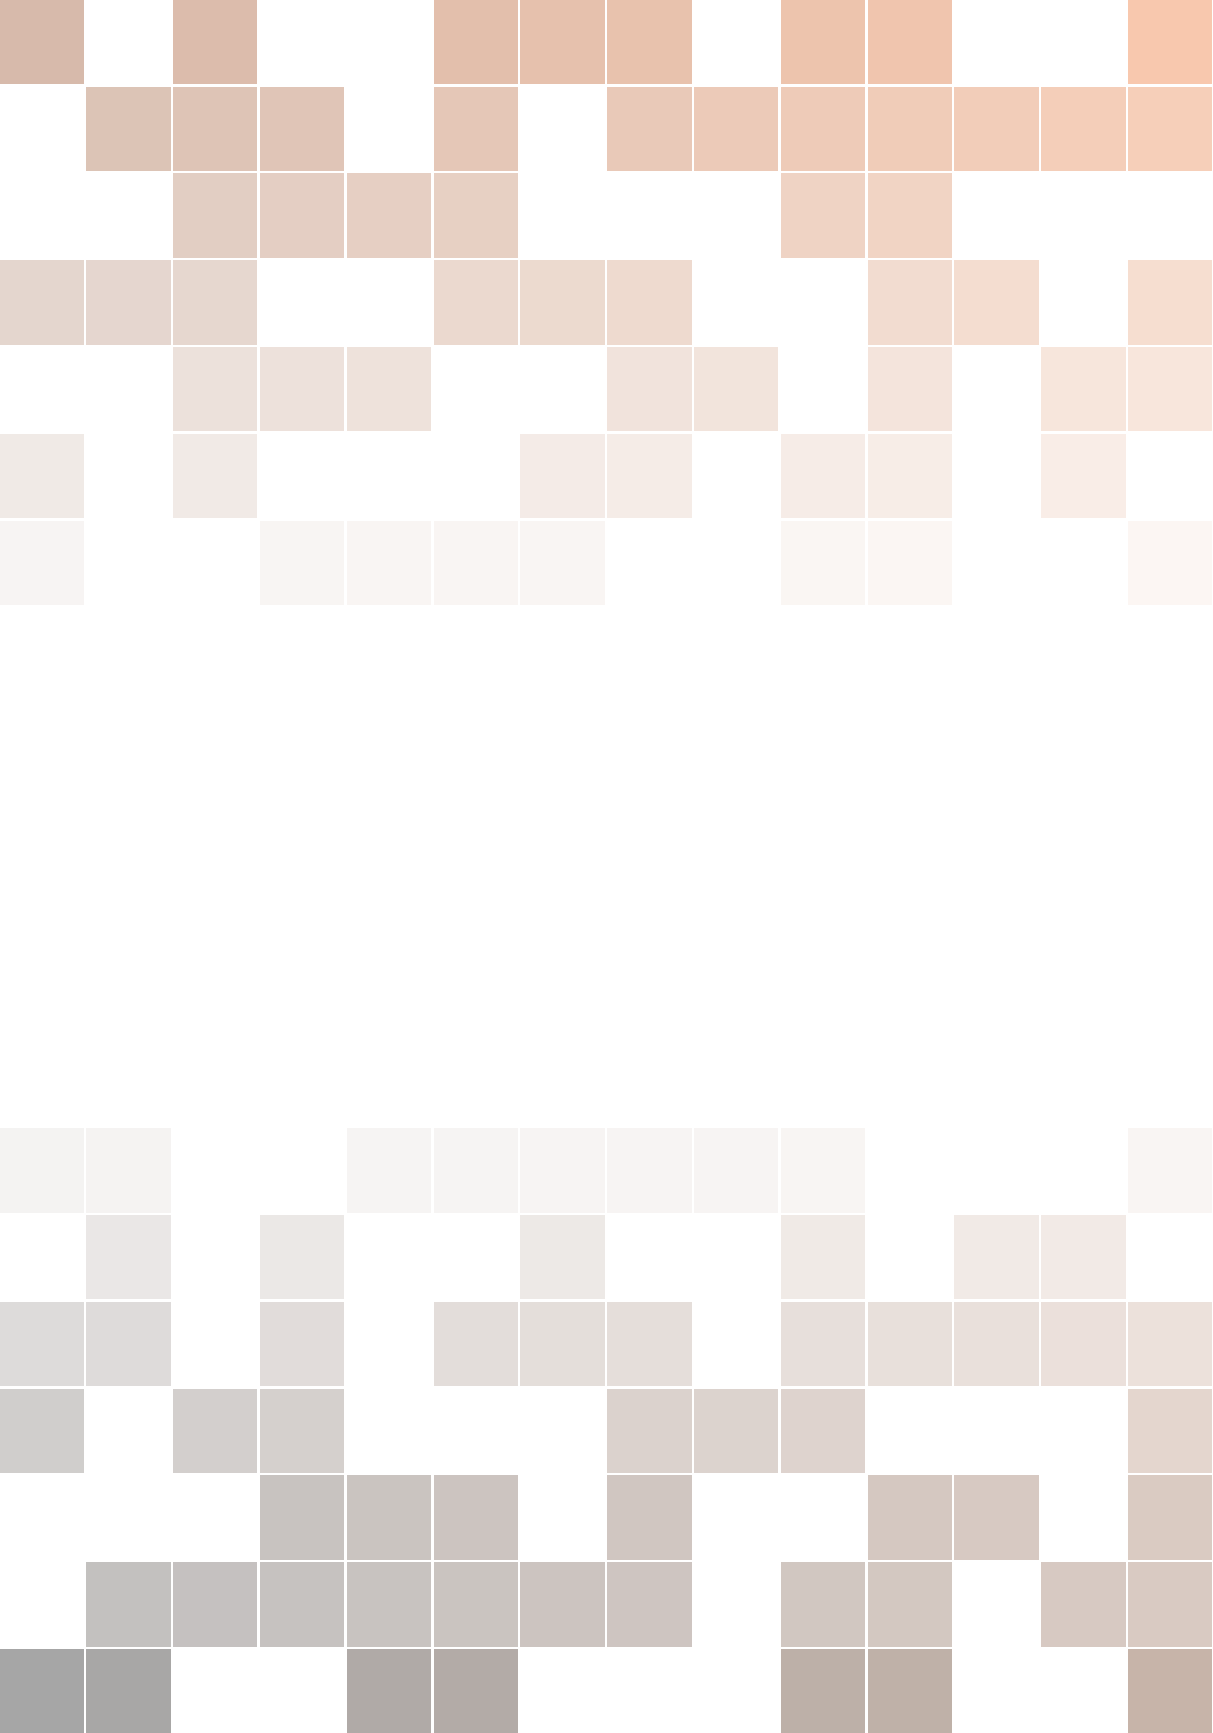
\includegraphics[width=\paperwidth]{background}}; % Background image
\draw[anchor=north] (midpoint) node [fill=ocre!30!white,fill opacity=0.6,text opacity=1,inner sep=1cm]{\Huge\centering\bfseries\sffamily\parbox[c][][t]{\paperwidth}{\centering Research report\\[15pt] % Book title
% {\Large A Profound Subtitle}\\[20pt] % Subtitle
{\Large Arnaud Bletterer}}}; % Author name
\end{tikzpicture}};
\end{tikzpicture}
\vfill
\endgroup

%----------------------------------------------------------------------------------------
%	COPYRIGHT PAGE
%----------------------------------------------------------------------------------------

\newpage
~\vfill
\thispagestyle{empty}

%----------------------------------------------------------------------------------------
%	TABLE OF CONTENTS
%----------------------------------------------------------------------------------------

\usechapterimagefalse % If you don't want to include a chapter image, use this to toggle images off - it can be enabled later with \usechapterimagetrue

\chapterimage{chapter_head_1.pdf} % Table of contents heading image

\pagestyle{empty} % No headers

\tableofcontents % Print the table of contents itself

\cleardoublepage % Forces the first chapter to start on an odd page so it's on the right

\pagestyle{fancy} % Print headers again

%----------------------------------------------------------------------------------------
%	CHAPTER 2
%----------------------------------------------------------------------------------------

\chapter{Semi-regular Surface Reconstruction}

This chapter explains a new method in surface reconstruction, based on the original data coming from many 3D scanners, namely depthmaps.

\section{Depthmaps}
Depthmaps are 2D grayscale images, representing the distance from points to the scene. They are a discrete local parameterization of the scene acquired using the scanners.

\subsection{Depthmaps reprojection}
There are many different methods to recover 3D positions from depthmaps, depending on the acquisition devices.

\subsubsection{LiDAR scanners}
For LiDAR scanners for example, it is common to use spherical coordinates to store values in the depthmaps.
\arnaud{Adding explanation about laser pulse system}
Spherical coordinates \cite{Wal67} are a coordinate system used to define positions over a sphere. 
They define $\theta$ to be the azimuthal angle $0 \leq \theta < 2\pi$ from the x-axis, $\phi$ to be polar angle (zenithal angle) $0 \leq \phi \leq \pi$ and $r$ to be the distance (radius) from a point to the origin $r \in [0;+\infty)$.

They are obtained from Cartesian coordinates by the following relations : 

\begin{equation}
\label{eq:cartesian_to_spherical}
	r = \sqrt{x^2 + y^2 + z^2} \\
	\theta = \tan^{-1}(\frac{y}{x})\\
	\phi = \cos^{-1}(\frac{z}{r}),
\end{equation}

and Cartesian coordinates can be recovered from those using : 

\begin{equation}
\label{eq:spherical_to_cartesian}
	x = r\cos\theta\sin\phi\\
	y = r\sin\theta\sin\phi\\
	z = r\cos\phi
\end{equation}

In depthmaps, the intensity stored for each pixel is the value of $r$. Knowing $\Delta\theta$ and $\Delta\phi$ (representing the difference of azimuthal and polar angles respectively between two consecutive points), one can recover $\theta$ and $\phi$ for each pixel of the depthmap, taking in consideration the structure of the depthmaps (2D matrices). 
Using Equation\eqref{eq:spherical_to_cartesian}, it is possible to recover 3D positions of points from intensity values contained in the depthmaps.

\section{Introduction}
\label{sec:introduction}

\section{Related work}
\label{sec:related_work}

Nowadays scanners are able to sample scenes with hundreds of million of points. Such amount of samples makes the surface reconstruction and visualization a challenging problem.
Specific surface reconstruction algorithms 

To resolve the interactive visualization problem, one common approach used is to modify the connectivity of the reconstructed mesh, in order to be able to easily decimate and refine it, depending on the distance of the visualization of the object to the viewer.
To do so, most of the methods find a parameterization of the mesh, and from a coarse approximation of the original mesh, which is called the base mesh, subdivide recursively triangles of this base mesh and reproject points over the original surface. A survey has recently been done to categorize the different methods \cite{PRS15}.
However this method requires to find a "good" parameterization of the surface, which can be a difficult problem, especially when it comes to handle objects having a really high gender.
Moreover, this introduces a remeshing error between the reconstructed mesh and the remeshed one.

Many 3D acquisition devices do not only provide a 3D point cloud at the output of an acquisition. They can also provide 2D parameterizations of a scene from the point of view of a scanner during the acquisition process, in the form of a depthmap (Figure \ref{fig:depthmap_point_cloud}(a)).

Depthmaps are 2D images, where each pixel represent a point in the scene acquired. This particular structure offers a natural connectivity through the point cloud, where neighboring pixels represent neighboring points on the acquired surface.
Taking this information in consideration, it seems natural to consider this connectivity when it comes to reconstruct the surface underlying the point cloud. 
In this method, we will show a method to reconstruct a semi-regular surface reconstruction algorithm, taking as an input a depthmap and a parametrization function, and reconstructing a semi-regular mesh.
The particularities of the method is that every step is applied in the parametric domain, which simplifies most of the algorithm applied, and the surface is only embed in 3D at the end of the algorithm, using the associated parametrization function.

\begin{figure}[ht]
\centering
\includegraphics[scale=0.05]{DepthMap-Garuda}
\centering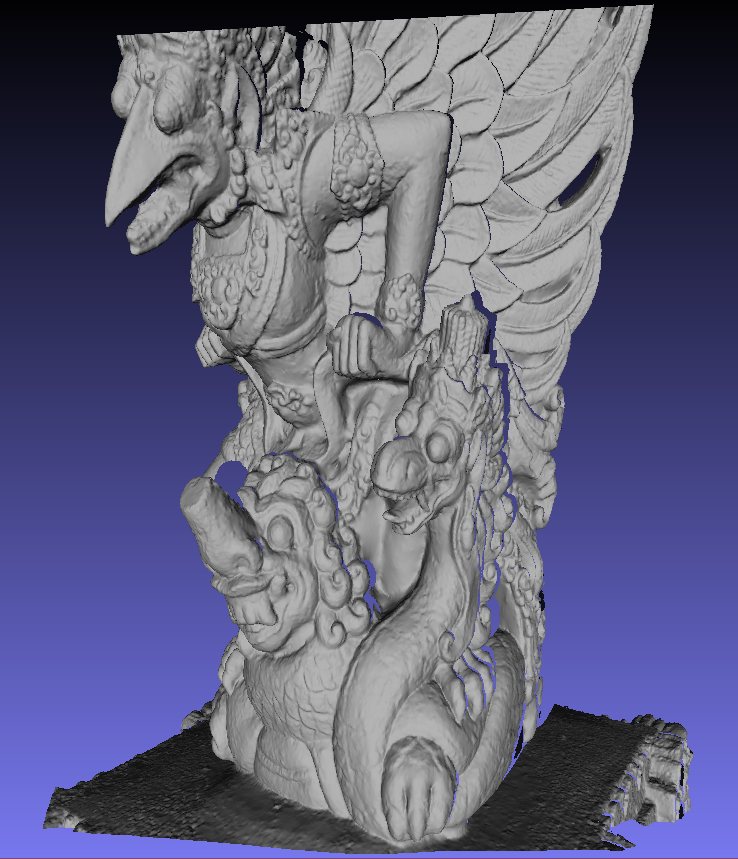
\includegraphics[scale=0.12]{PointCloud-Garuda}
\caption{Example of a depthmap (a) (darker colors represent closer points to the scanner) and the point cloud representing the embedding of the depthmap in 3D (b) (normals have been computed to enhance the visualization).}
\label{fig:depthmap_point_cloud}
\end{figure}


\section{General overview}
\label{sec:general_overview}

Figure \ref{fig:general_steps} represents the different steps of our method used to reconstruct a semi-regular surface mesh from a depthmap.

\begin{figure}[ht]
\centering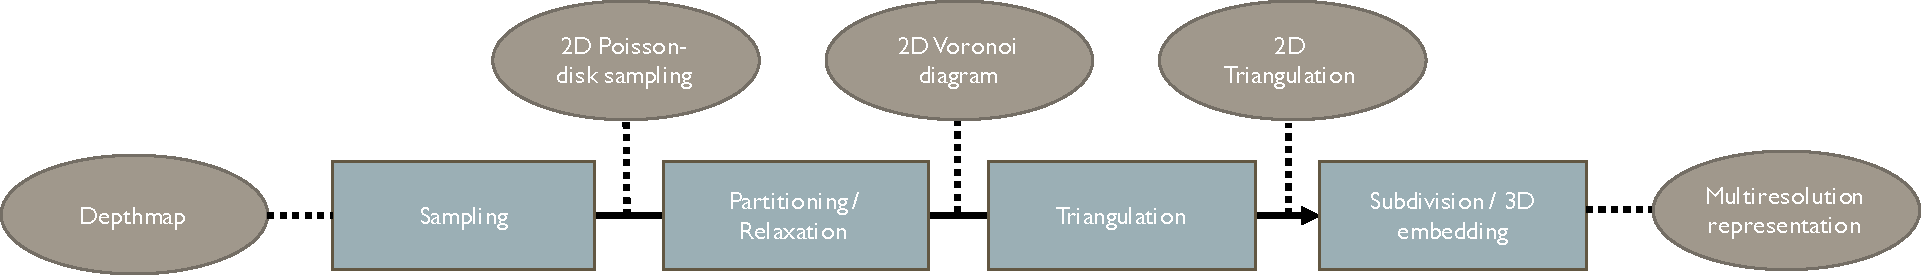
\includegraphics[scale=0.46]{MethodPipeline}
\caption{General steps of our algorithm}
\label{fig:general_steps}
\end{figure}

A Poisson-disk sampling is applied on the depthmap (Section \ref{sec:poisson_sampling}) that will generate the initial sites for a Lloyd relaxation procedure (Section \ref{sec:lloyd_relaxation}). 
Then the obtained Voronoi diagram will be transformed into a 2D triangulation, considering an altered dual representation (taking into account parts identified of the depthmap where two neighboring pixels represent points on different surface areas (Section \ref{sec:border_marking})). 
Finally, from this 2D triangulation, different levels of resolution are reconstructed using a 1-to-4 face subdivision approach (Section \ref{sec:surface_subdivision}).
Finally the reconstructed surface is obtained by embedding the different 2D triangulations obtained in 3D.

\section{Border marking, labeling and routing}
\label{sec:border_marking}

A depthmap is a 2D parameterization of a 3D scene visualized from a specific point of view. From this representation it is possible to obtain a point cloud representing the samples acquired from this specific point of view (Figure \ref{fig:depthmap_point_cloud}(b)).

This link between depth values and 3D coordinates motivated us using depthmaps as a parameterization domain to apply algorithm on point clouds, considering the implicit connectivity between pixels to do local computations requesting the consideration of neighboring points.

If most of the time it is correct to consider that neighboring pixels in a depthmap are also neighbors on the surface (with respect to the sampling density of the acquisition), it is not the case along depth discontinuities (Fig \ref{fig:depth_discontinuity}).
Since an acquisition is done from a specific position and orientation, it can only represent visible points from that specific point of view. 
Thus many surface areas can be occluded, and different surface areas could be considered touching each other in the depthmap, even if they are far on the surface.

To avoid this, we present a method to mark the borders, identify each of them uniquely and store the path from the beginning until the end of each border.

Many methods have been developed to detect borders and to segmentate  however those techniques only want to separate different areas of the image, or image parts where specific processing should be applied.
In our case, we not only want to detect borders, we also want to store the path that each border follows.

\begin{figure}
\centering
\scalebox{0.05}{
\begin{tikzpicture}[spy using outlines={circle,red,magnification=10,size=50cm, connect spies}]
\node {\pgfimage{Images/DepthMap-Garuda}};
\spy on (5,-1) in node [left] at (100,0);
\end{tikzpicture}
\begin{tikzpicture}[spy using outlines={circle,red,magnification=10,size=50cm, connect spies}]
\node {\pgfimage{Images/Borders-Garuda}};
\spy on (5,-1) in node [left] at (100,0);
\end{tikzpicture}
}
\caption{High depth variation between neighboring pixels that do not belong to neighboring surface areas (left), and the detected associated borders (right).}
\label{fig:depth_discontinuity}
\end{figure}

\subsection{Border marking}
First, we mark all the pixels of the depthmap that do not fulfill a local depth-discontinuity condition. We consider a depth-discontinuity as being an important change of depth in at least one direction (horizontal, vertical or diagonal).

During that step, we are defining how points would be triangulated if a mesh was going to be constructed between neighboring pixels over the whole depthmap. 
For this, we consider an arbitrary connectivity pattern, connecting one pixel to 6 of its neighbors, and will use that pattern to consider the possible neighbors of a point (Figure \ref{fig:pixel_neighborhood}). 
This pattern will be used during the following neighborhood considerations.

\begin{figure}[ht]
\centering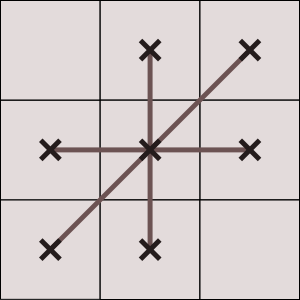
\includegraphics[scale=0.4]{PixelNeighborhood}
\caption{The 6-neighborhood considered around each pixel}
\label{fig:pixel_neighborhood}
\end{figure}

For each pixel $p$, we search to know if there a high intensity variation with respect to each of his neighbors. If this is the case, it means that the two pixels do not belong the same surface area, and then need to be separated for the further processings.
But instead of using a fixed threshold over the entire depthmap, we consider a variable parameter, which value will vary with respect to the distance from the camera.
This comes from the fact that 3D scanners acquires a higher density of points when objects are closer than when they are further. 
Thus by weighting a chosen threshold with pixel intensities, we are able to have a threshold that will vary with respect to the depth, i.e it will be smaller for high density areas, and bigger for low density areas.

Since this is a highly parallelizable algorithm (each operation is executed indepently for each pixel), we implemented it using GPGPU methods.

\subsection{Border labeling and routing}
Now that borders have been indentified, we need to label them in order to be able to consider them independently. 

Each border is represented as a list, characterizing the path from pixel to pixel, from the beginning until the end of the border.

We decide to use a region-growing process. 
Starting from a pixel that has been marked as a border, we try to find the next pixel defining the same border. 
This is equivalent as searching the next vertex along the border of the triangulation, considering oriented faces.
When this vertex has been found, it is added to the current border list, and being processed, to find the next pixel of the border after him.
When there is no more pixel than can be added to the current border, the border is considered as completed.

At the initialization, every pixel marked as a border is added to a list. Until the list is not empty the first pixel is treated and removed from the list. 
If the pixel has already been labeled, then it is ignored, and the next one is considered instead. 
If the pixel isn't already labeled it is used as the starting pixel of a new border, following the steps.

\begin{figure}[ht]
\centering
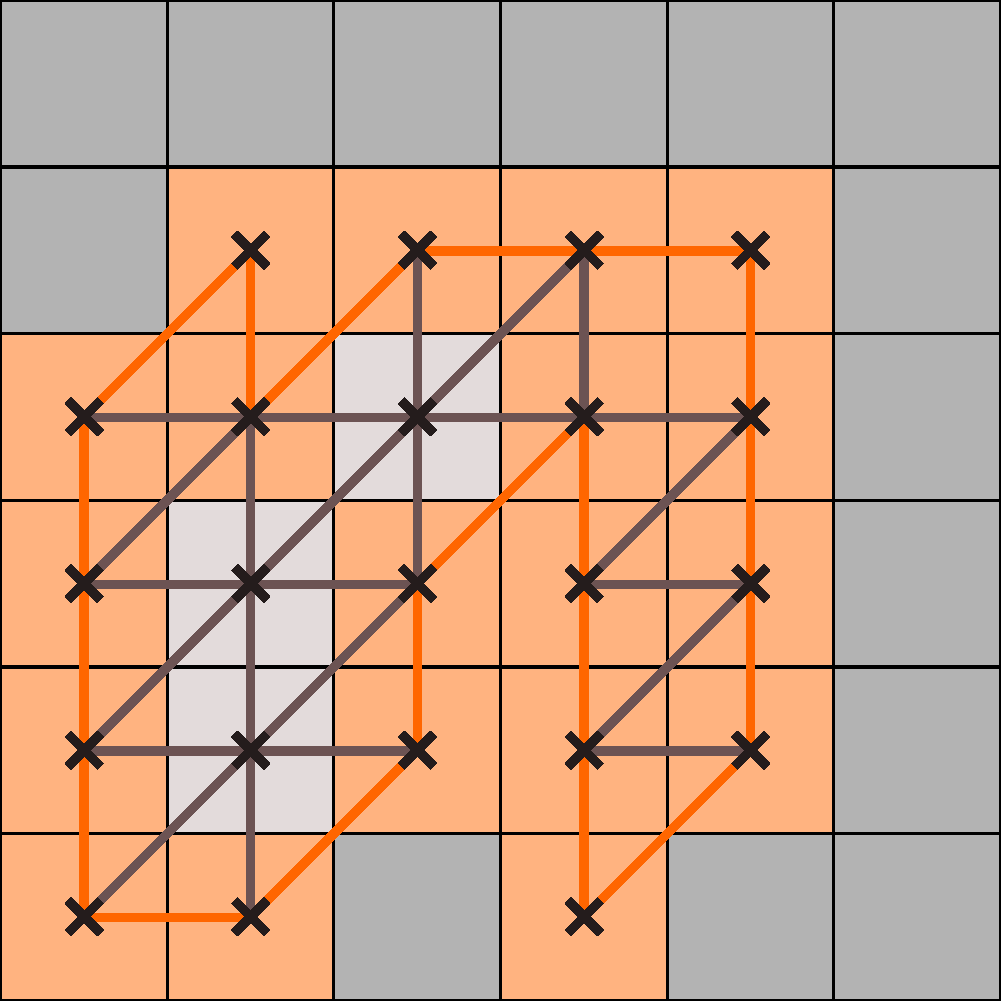
\includegraphics[scale=0.3]{PixelTriangulationBorder}
\caption{Implicit triangulation of a depthmap constructed when finding the border pixels. Darker pixels represent background, lighter and orange represent the object, and orange pixels alone represent the pixels marked as "borders".
Edges in orange are the edges defining the border of the triangulation.}
\label{fig:border_triangulation}
\end{figure}

\section{Poisson-disk sampling of the depthmap}
\label{sec:poisson_sampling}

In semi-regular triangle remeshing, to construct a semi-regular mesh from an irregular one, one method consists in constructing a base mesh, i.e. a low resolution version of the irregular one and subdividing it recursively (and projecting the generated vertices onto the original surface) \cite{PRS15}. Our work is inspired by those methods, constructing first the base mesh (from a set of samples acquired on the surface, i.e pixels on the depthmap) and the reconstructing the different levels of resolution.

To obtain a good distribution of the base vertices over the depthmap, we use a poisson-disk sampling, as it has been shown to be one of the best sampling patterns for many applications. 
We use a dart-throwing approach to choose the samples, combined with an region-growing process through Dijkstra's algorithm \cite{Dij59} to compute the disks areas.
We compute a connectivity graph over the depthmap. Each pixel can have up to 6 neighbors (with respect to the triangulation pattern chosen at the beginning).
An edge is created between every pair of neighboring pixels, only the ones being part of different borders are not connected together. 
The weight of each edge is chosen depending on the metric considered.

\subsection{Uniform sampling}
This method uses the 3D coordinates of points (where each point is a pixel embedded in 3D using the depth information stored at that pixel) and weights each edge using the euclidean distance between both points.
By using Dijkstra's algorithm, we can then construct the shortest path between a source (center of a disk) and any point of the domain. 
By using this method, we consider Poisson disks (surface patches to be more precise) that have an uniform area in 3D.

\begin{figure}[ht]
\centering
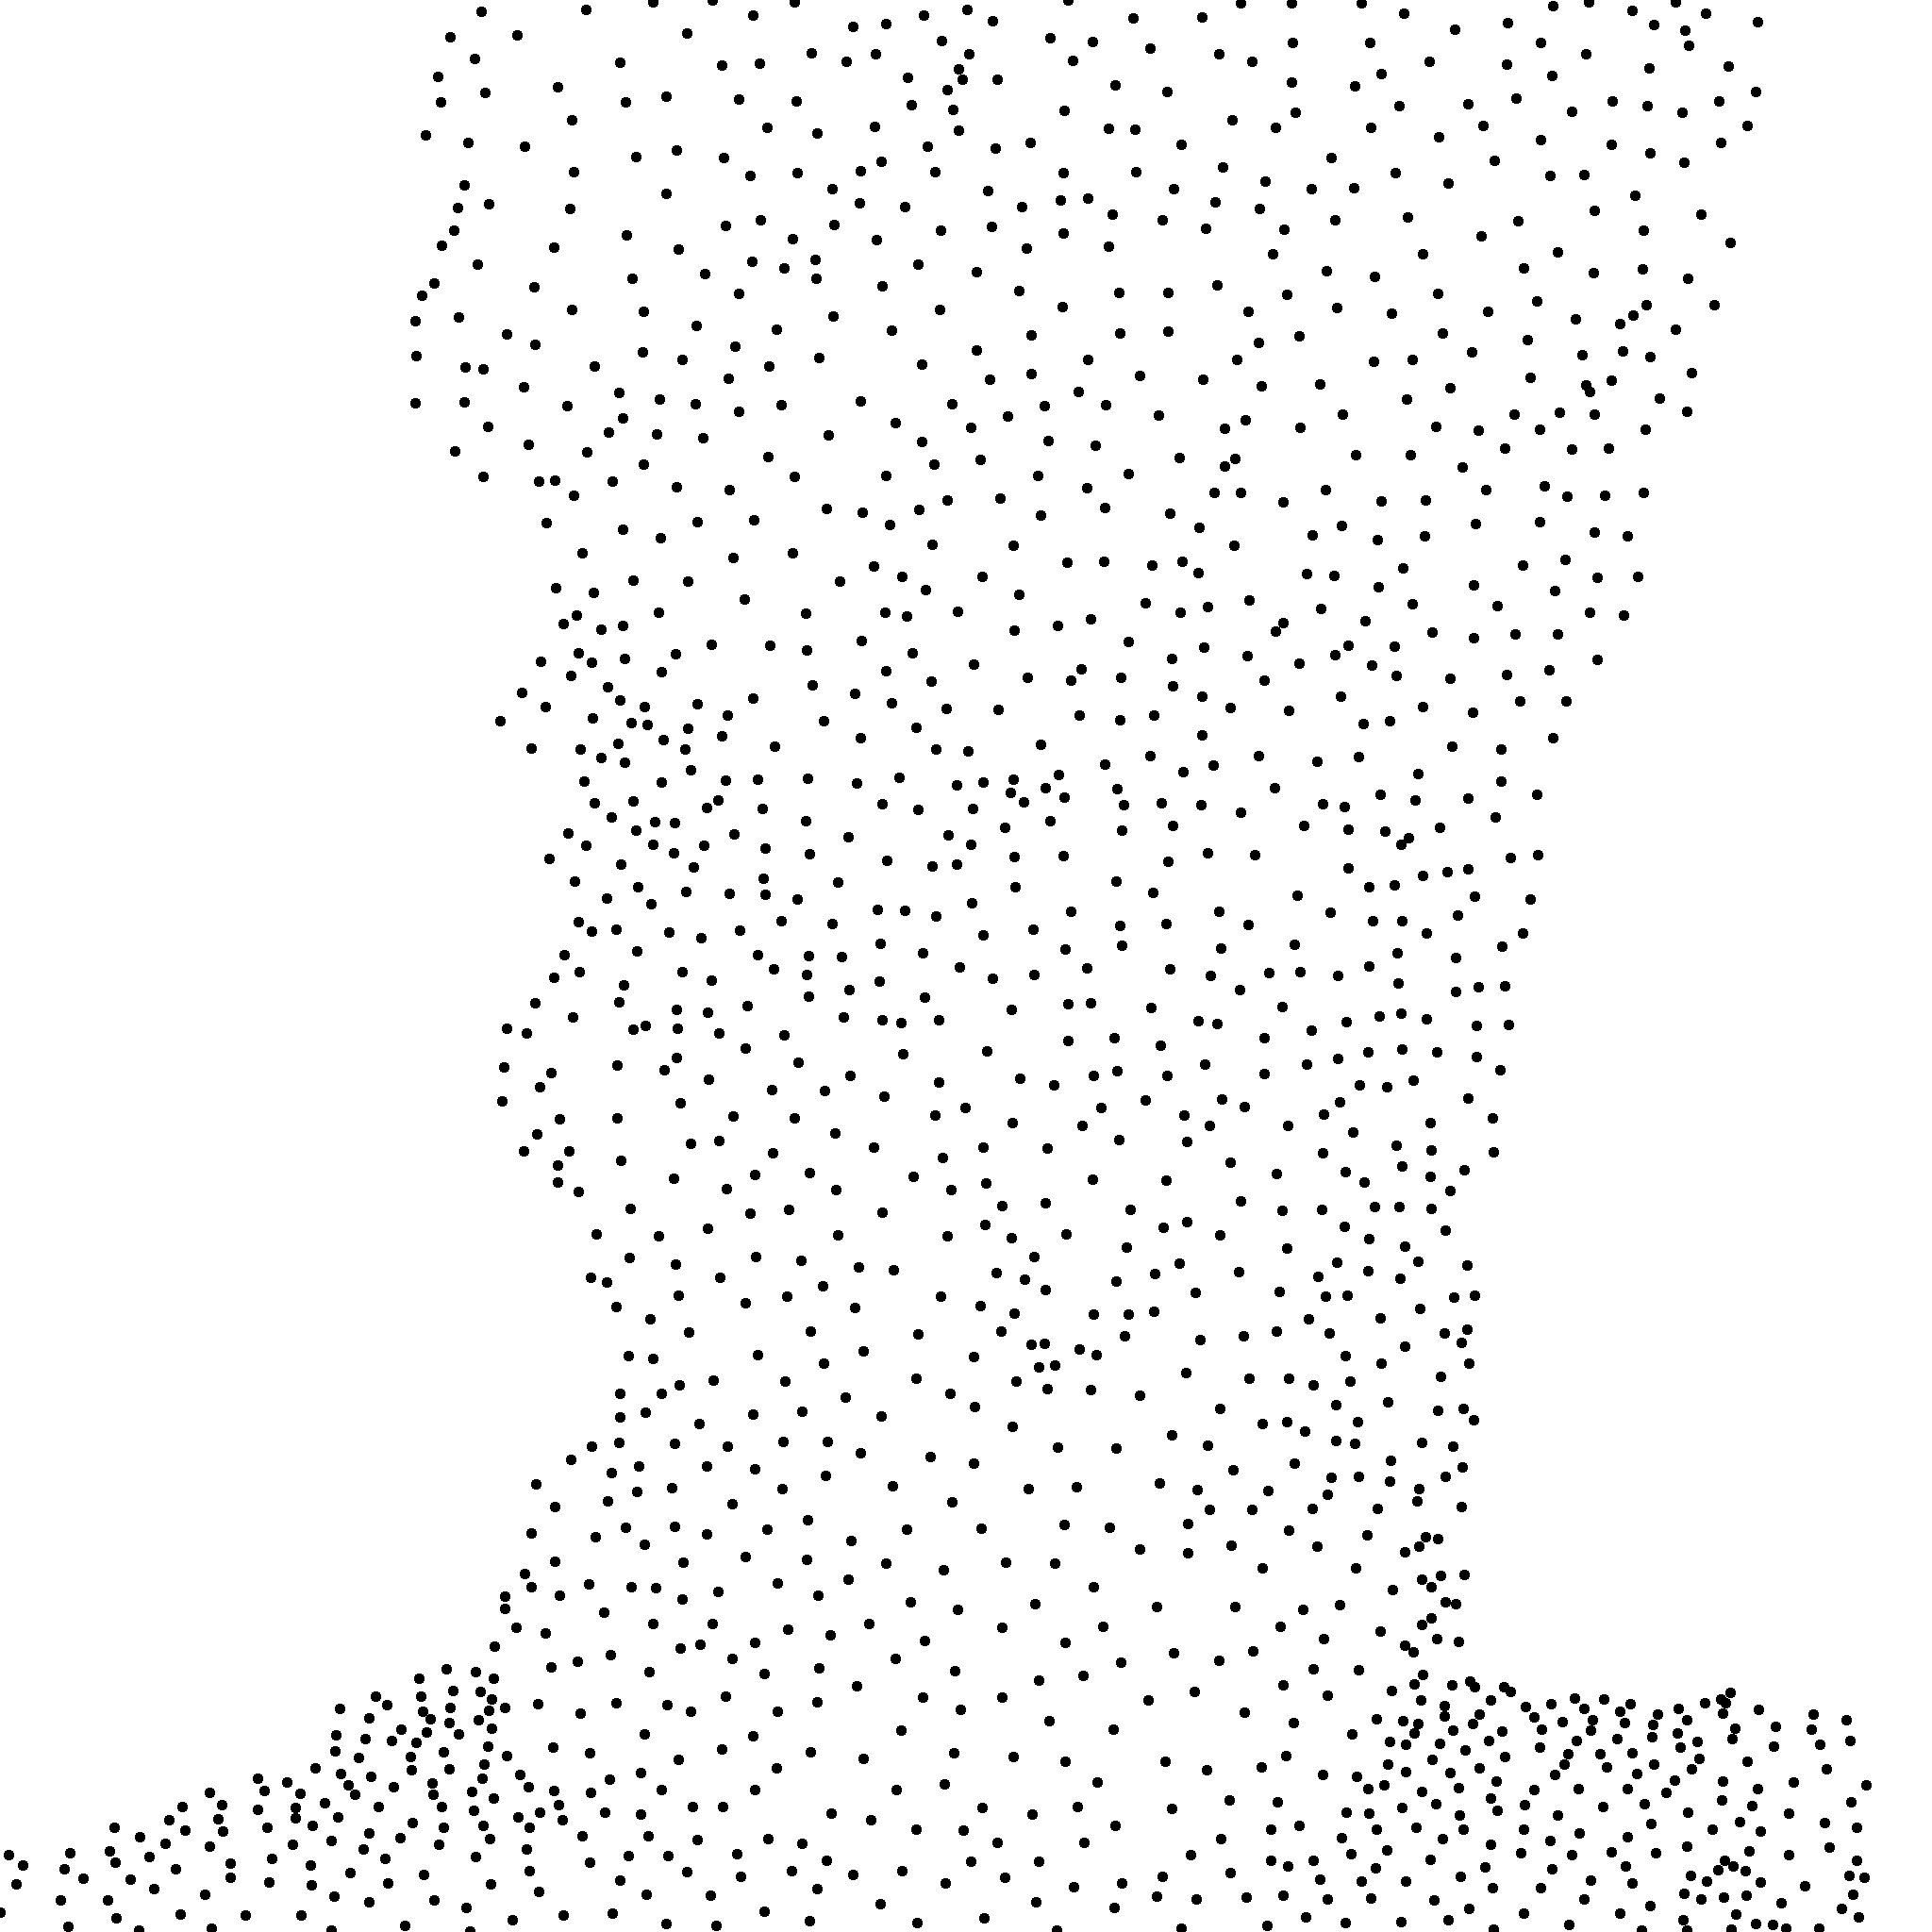
\includegraphics[scale=0.05]{PoissonSampling3D-Garuda}
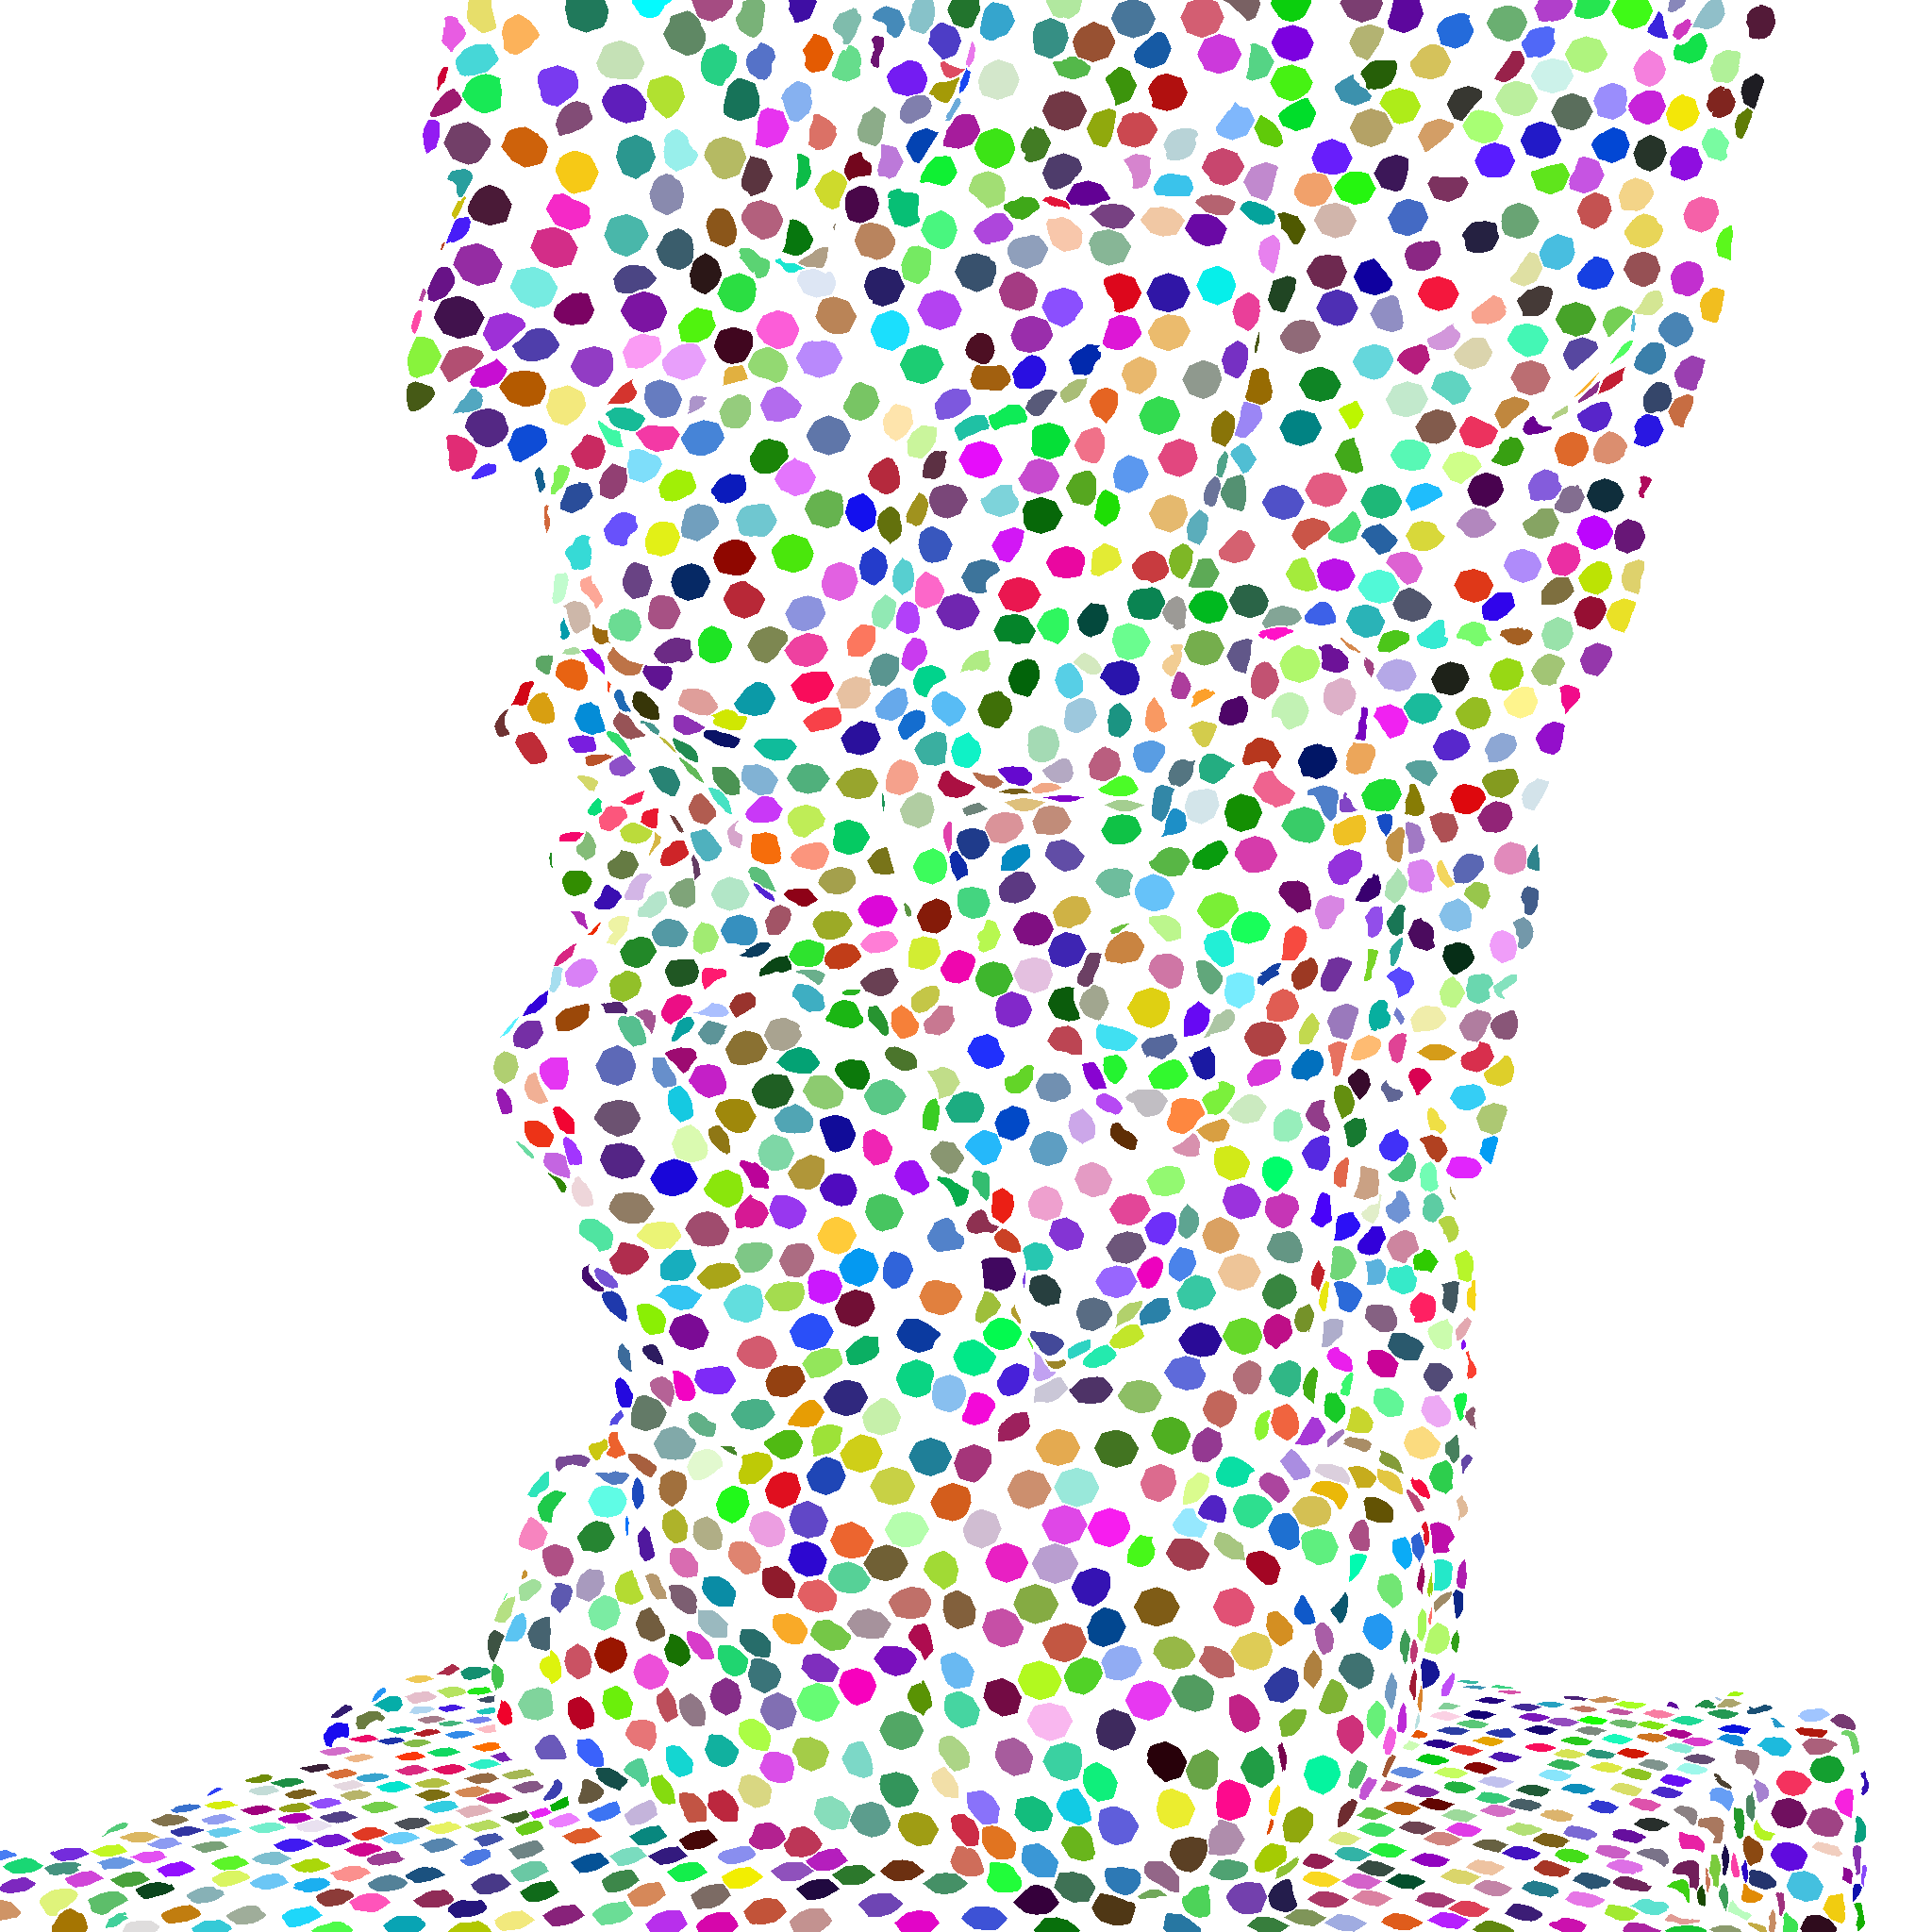
\includegraphics[scale=0.05]{PoissonDisks3D-Garuda}
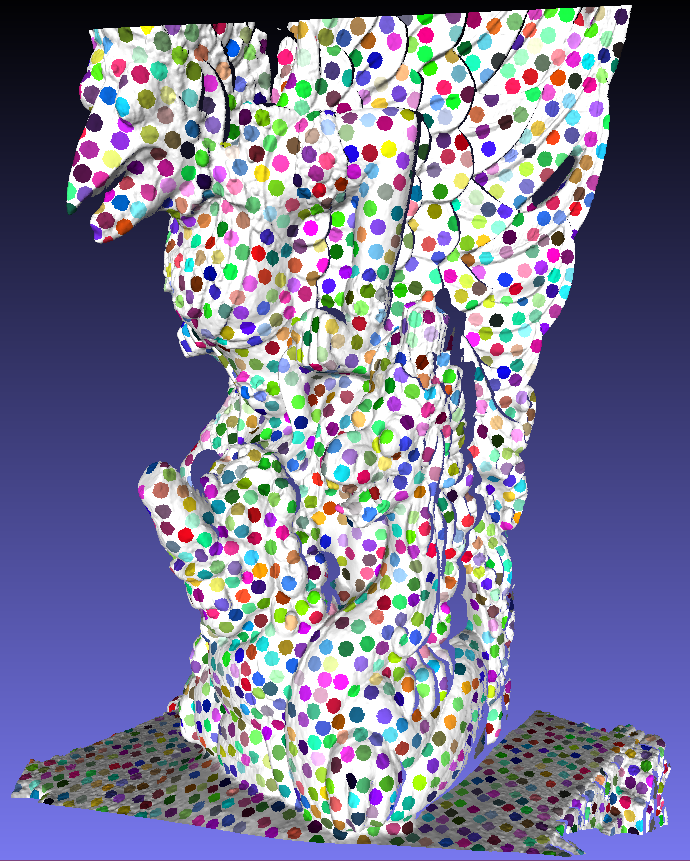
\includegraphics[scale=0.12]{PoissonDisks3DEmbedded-Garuda}
\caption{Poisson-disk sampling of the model Garuda considering disks with an uniform area in 3D (a) with their associated disks (b) and the same disks, but embedded in 3D (c)}
\label{fig:poisson_sampling_3d}
\end{figure}

\subsection{Density adaptive sampling}
Depthmaps can represent scenes having a really huge difference in sampling density, depending on the distance of a surface area to the scanner. 
For example, on the (Figure \arnaud{ADD FIGURE SHOWING THE SAMPLING DENSITY DIFFERENCE}) points in the green area have a sampling density of \arnaud{sampling density value w.r.t Bbox} and the pixels in the blue area have a sampling density of \arnaud{sampling density value w.r.t Bbox}. It can be interesting to conserve that difference of density when choosing the samples, in order to keep the precision of the original acquisition, when fine structures have been acquired.

Instead of sampling a point cloud uniformly in 3D, we suggest to take the local sampling density into account. In other words, rather than computing disks with an uniform radius in 3D, we constrain each disk to have an uniform radius in 2D.
Interestingly, this can easily be obtained by sampling the depthmap without considering 3D geodesic distances, i.e. doing a classical Poisson-disk sampling on an discretized planar domain, using a Dart Throwing approach for example.

\begin{figure}[ht]
\centering
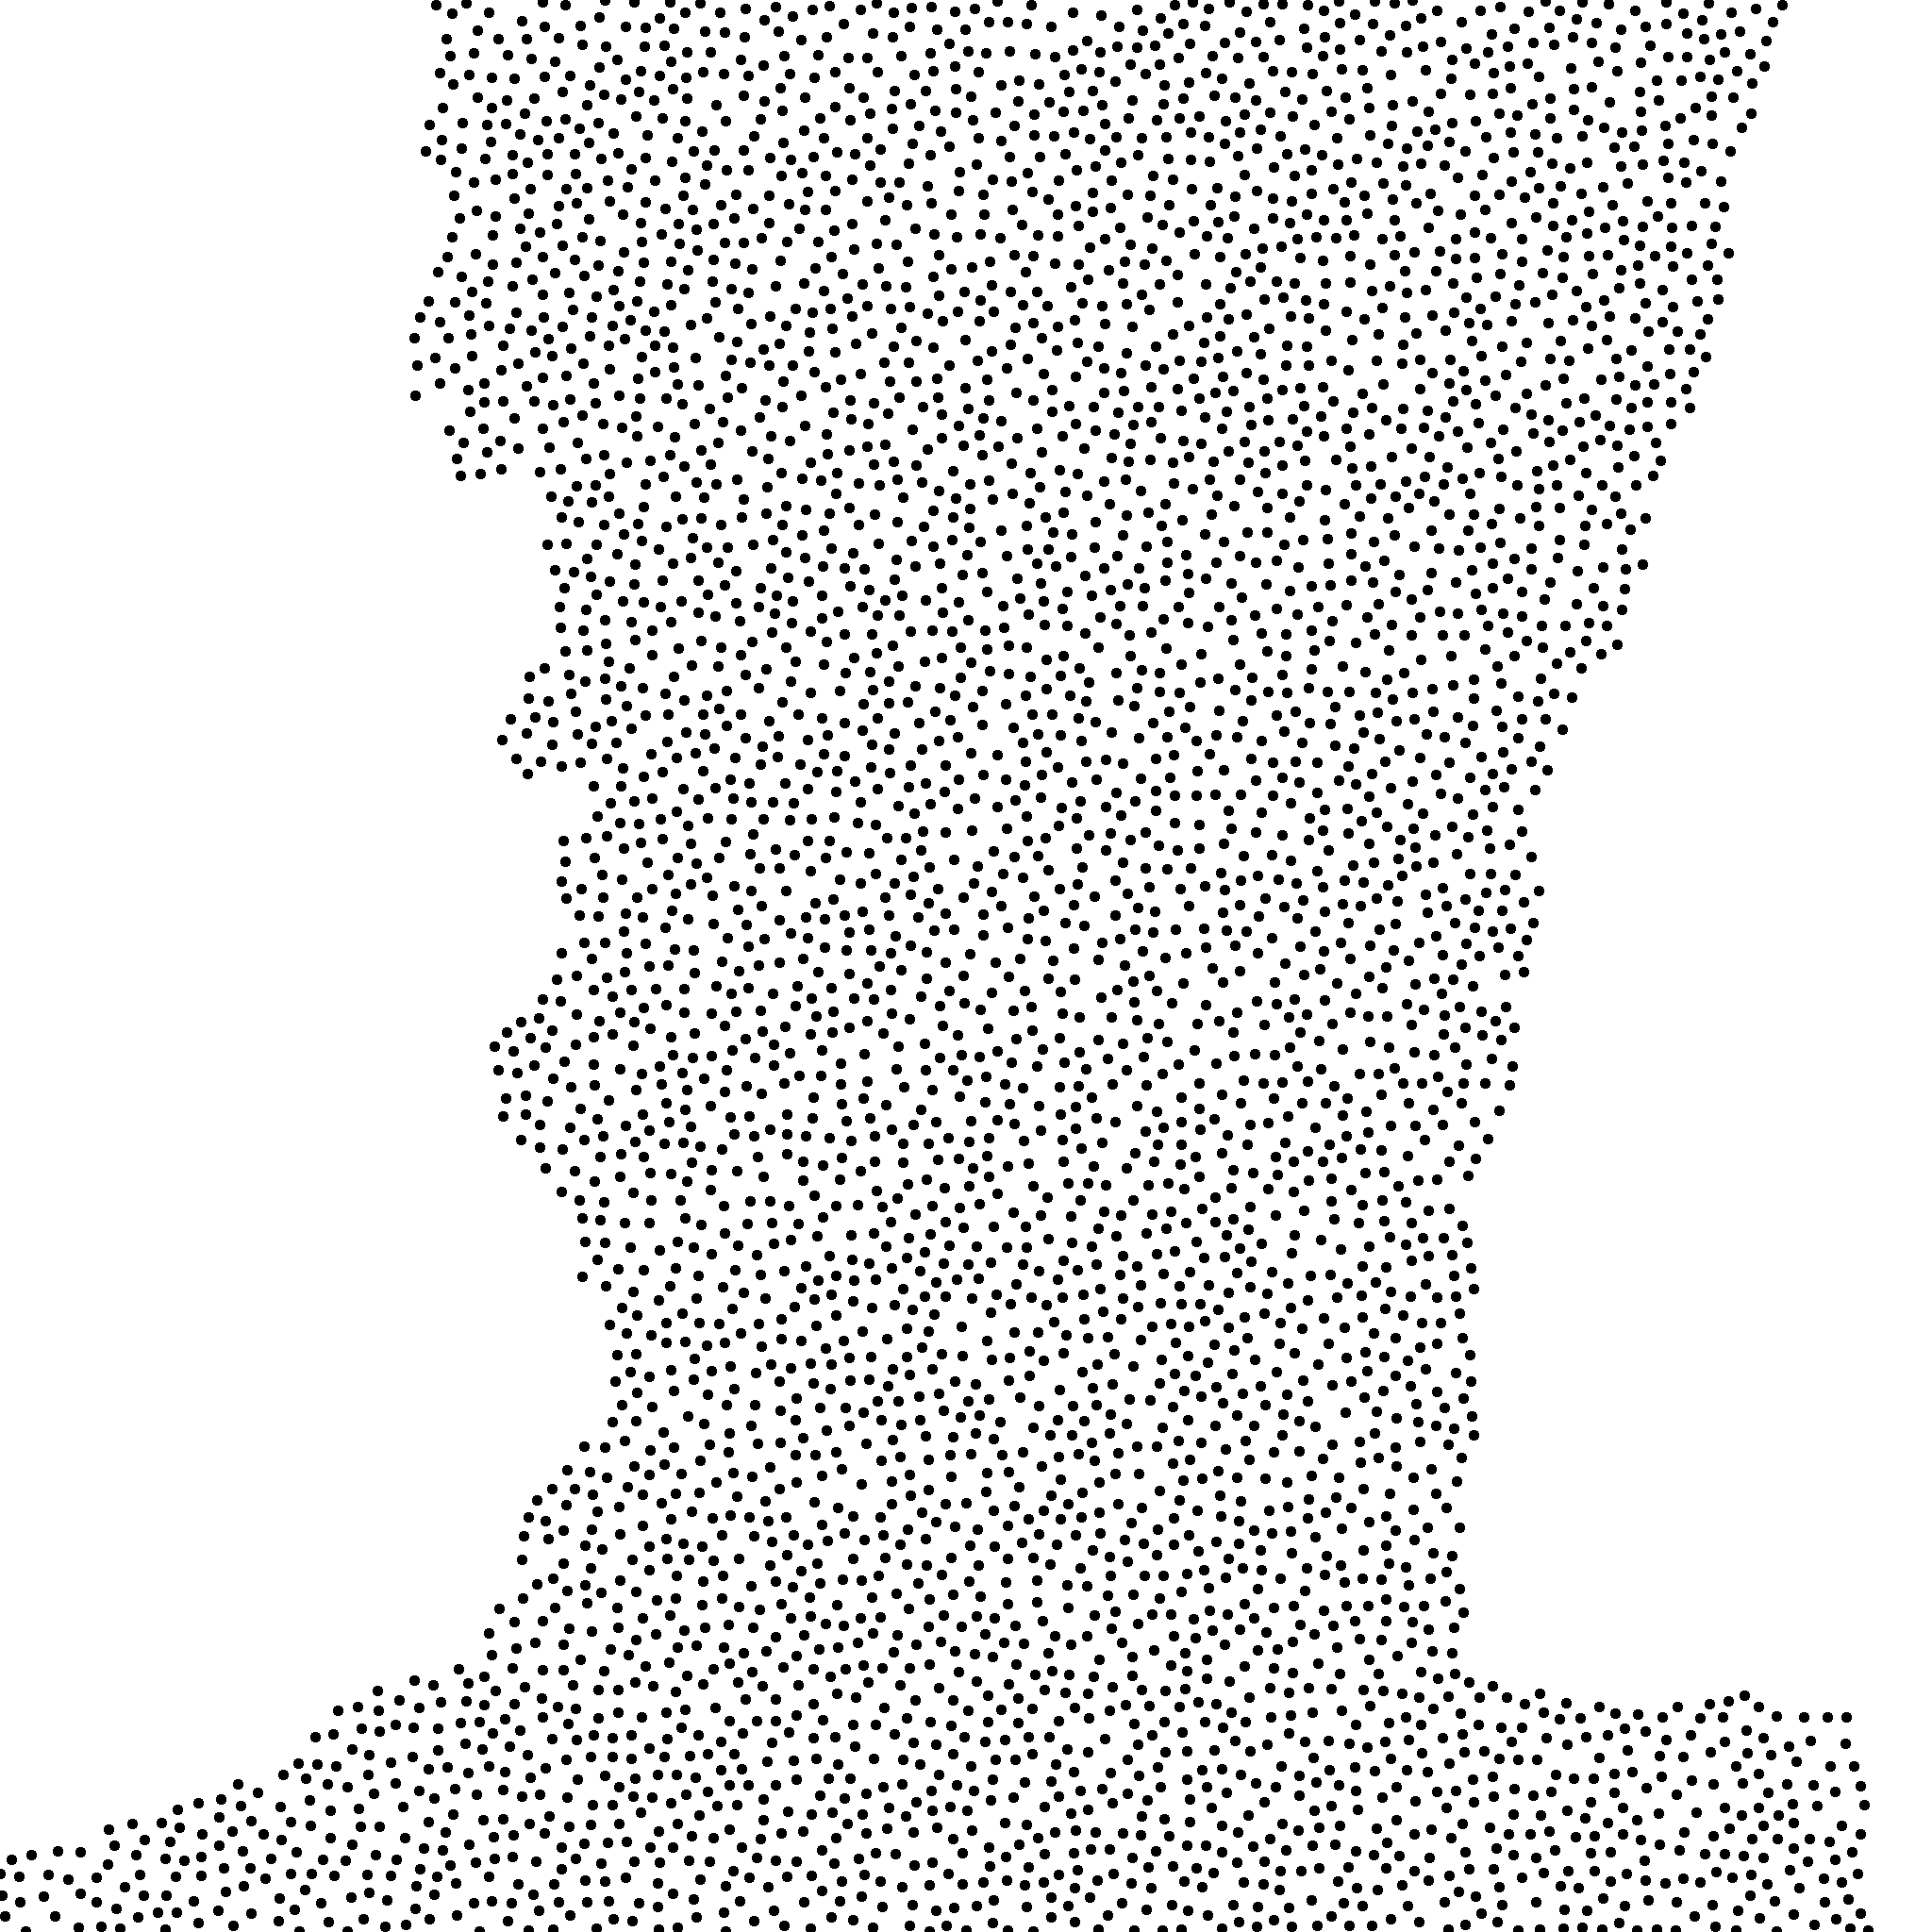
\includegraphics[scale=0.06]{PoissonSampling2D-Garuda}
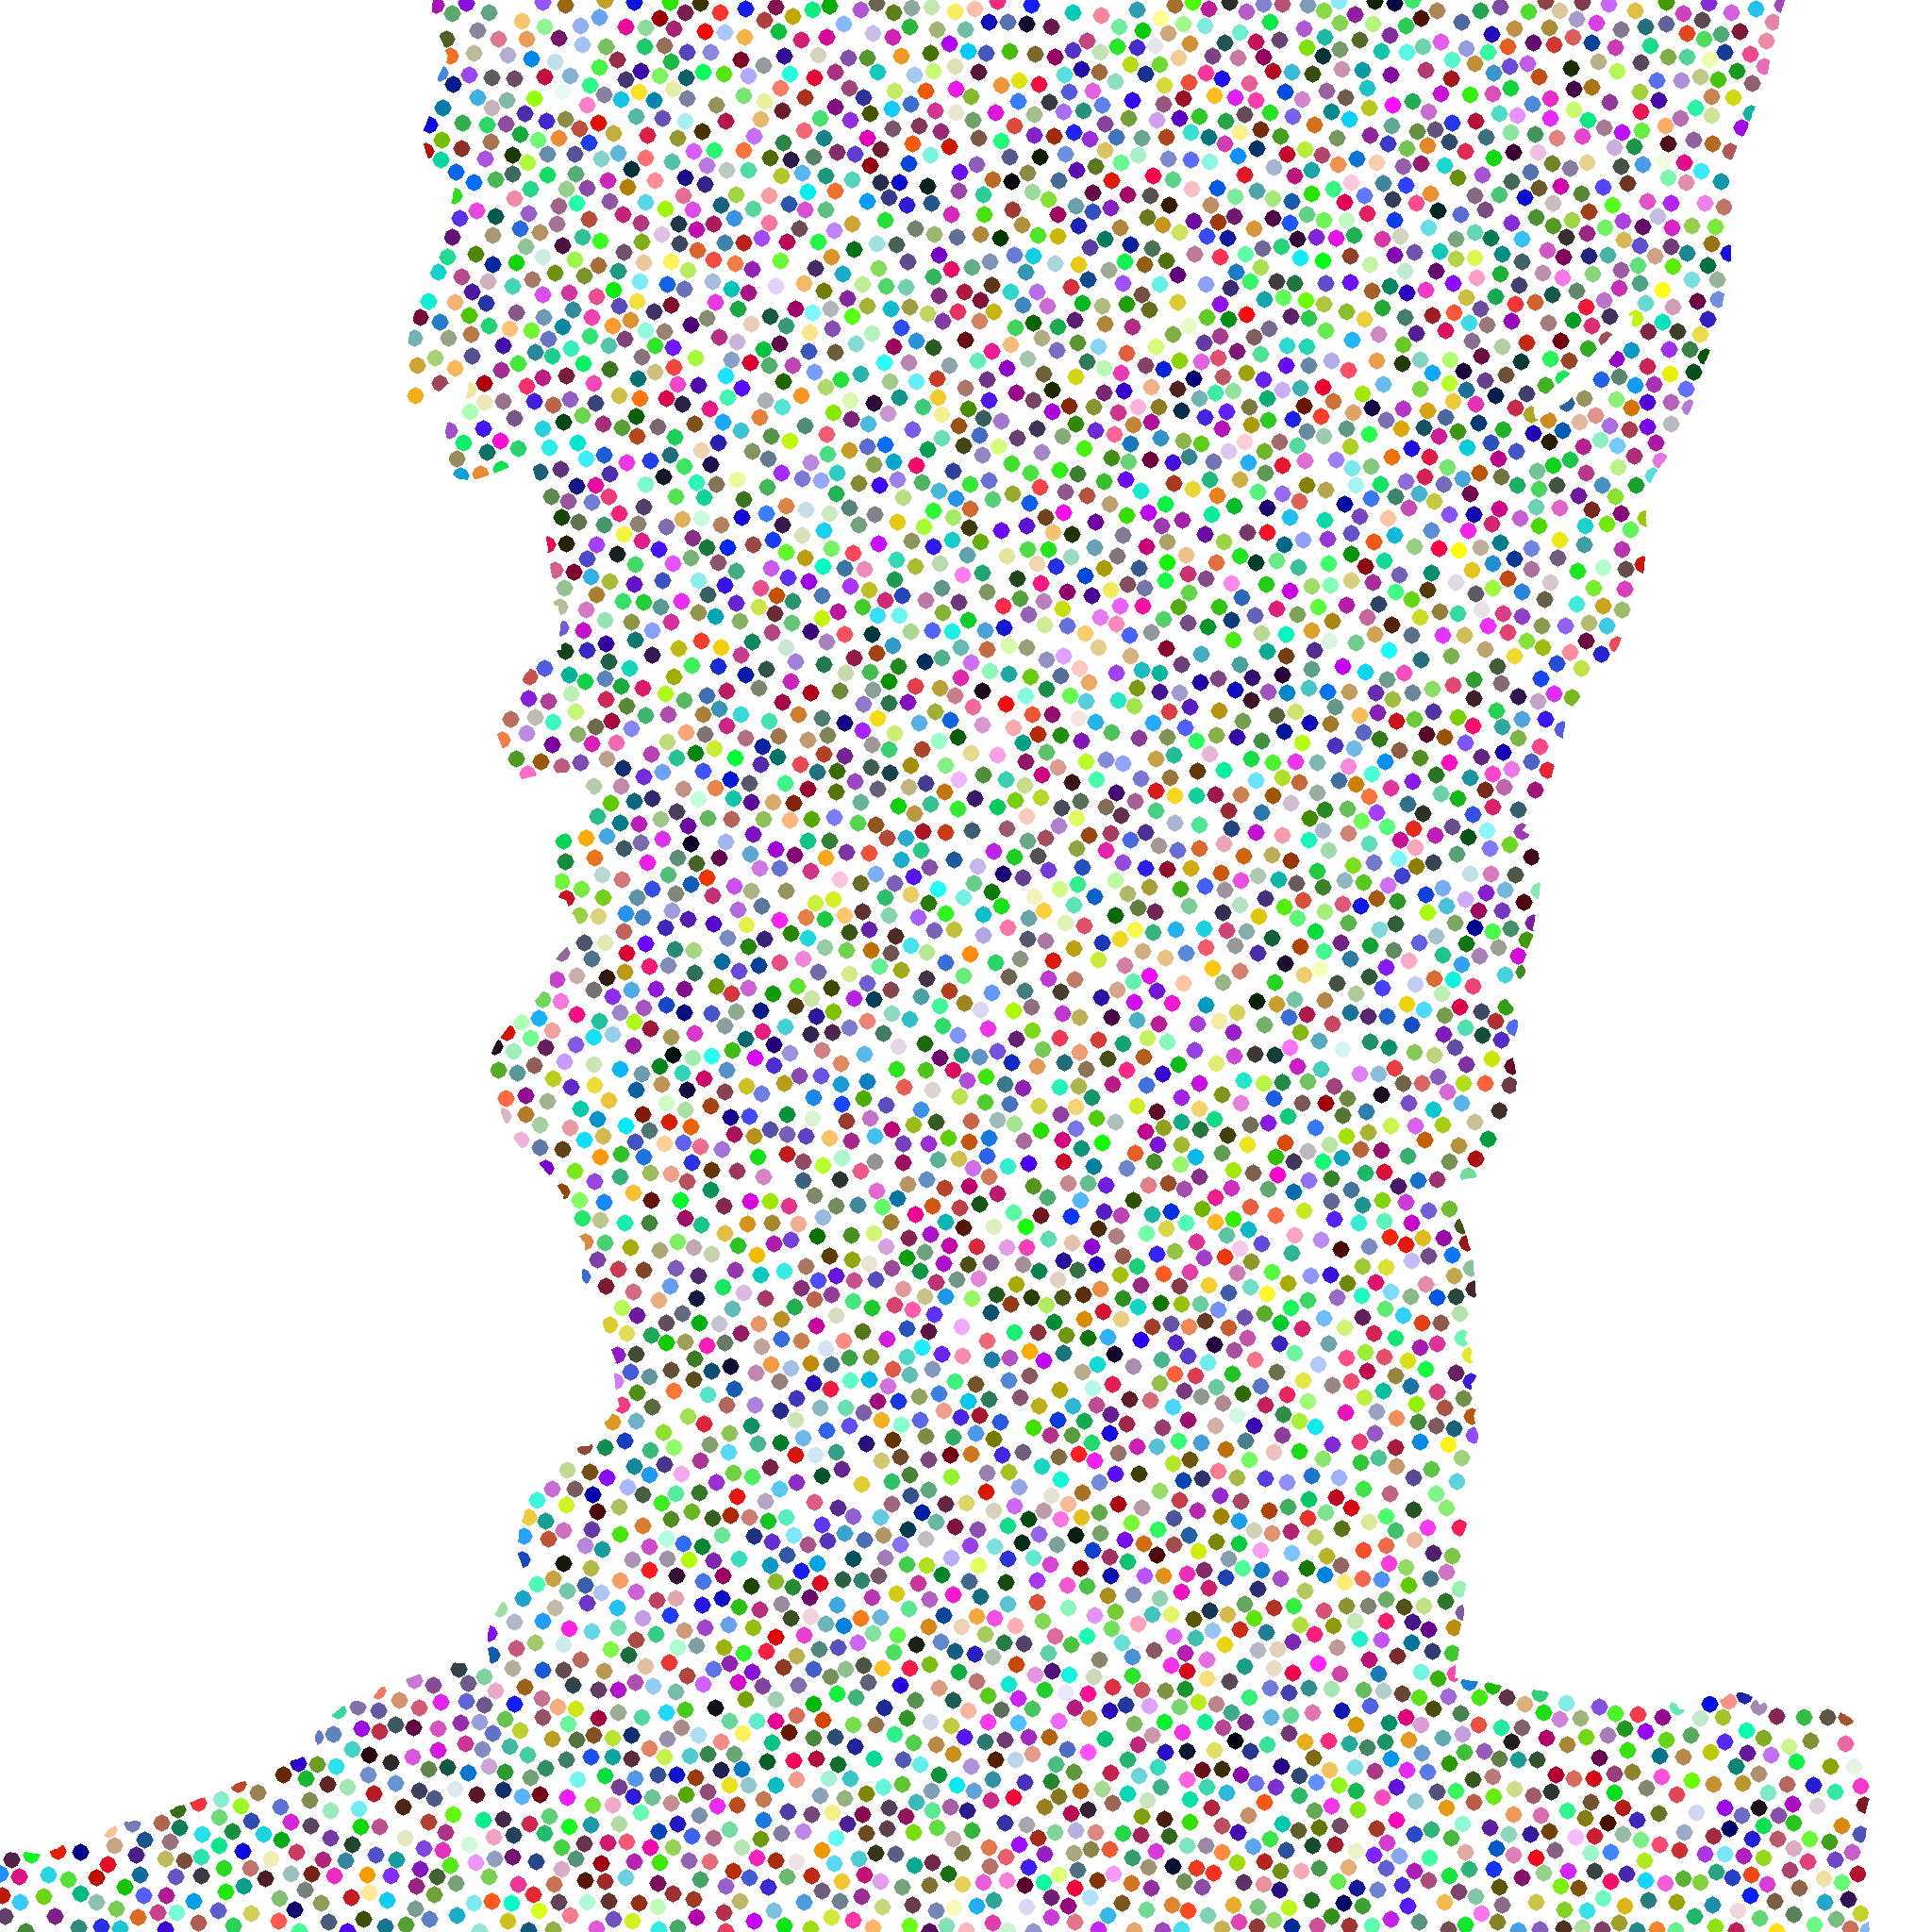
\includegraphics[scale=0.06]{PoissonDisks2D-Garuda}
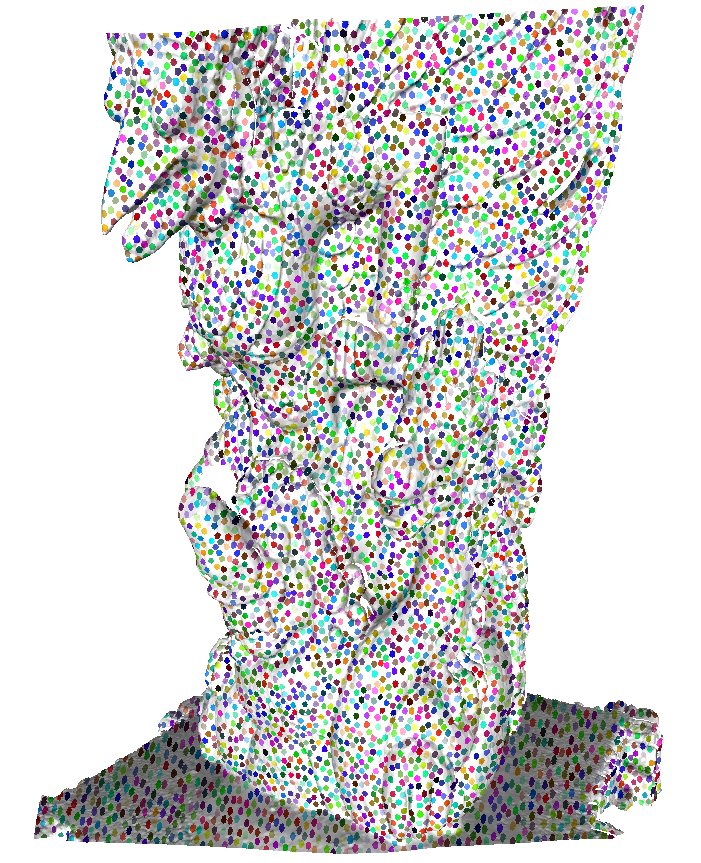
\includegraphics[scale=0.14]{PoissonDisks2DEmbedded-Garuda}
\caption{Poisson-disk sampling of the model Garuda considering disks with an uniform area in 2D. Samples found (a) with their associated disks (b) and the same disks, but embedded in 3D (c)}
\label{fig:poisson_sampling_2d}
\end{figure}

% \subsection{Curvature adaptive sampling}
% In order to preserve the fine details during the sampling process, it would be interesting to sample more densely the surface areas where the surface curvature is high (representing high changes in the normal field). For this, the idea is to consider the "normalized" Gaussian curvature as probability density function, giving a higher probability to points in areas of high absolute curvature, and a lower probability to points in areas of low absolute curvature.

% \arnaud{INSERT GEOMETRIC GAUSSIAN CURVATURE ADAPTIVE SAMPLING}
% \arnaud{Subsection incomplete, need an explanation on curvature estimation from the normals (so adding also an explanation on the normal computation using depthmap connectivity and 3D positions)}

\section{Voronoi diagram generation and Lloyd relaxation}
\label{sec:lloyd_relaxation}

In order to even the sites positions, we apply a Lloyd relaxation scheme based on 3D geodesic distances, using the connectivity of the depthmap.
This algorithm is decomposed into two steps : 
\begin{itemize}
	\item Computing a voronoi diagram, determining for each site $s_i$ the closest points from $s_i$ to any other site.
	\item Moving the position of each site $s$
\end{itemize}

Those steps are repeated until the sites stop moving (in practice, the process is stopped when the mean displacement is below a given threshold).

\subsection{Voronoi diagram generation}
Voronoi diagrams \arnaud{(add citation)} are a partition of a space $\mathbb{R}^n$ in a set of convex cells $V_S(v_i)$ from $k$ sites where every element contained in the cell $V_S(v_i)$ is closer from the site $v_i$ than from any other site $v_j$

\begin{equation}
\label{eq:voronoi_cell}
	V_S(v_i) = \{ x \in \mathbb{R}^n, \forall p \in S\, d(v_i,p) \leq d(v_j,p), j \neq i\},
\end{equation}

where $d$ is a distance metric. Generally, the euclidean distance metric is used to partition the domain, however it is possible to use other distance metrics (Manhattan distance, geodesic distance, ...), that will generate other partitions, depending on the needs.

To compute a Voronoi diagram over a depthmap, we use a discrete approach, through the multi-sources Dijkstra's algorithm (MSSP) \cite{Dij59} which finds for a vertex of a graph, the shortest path through the graph between this vertex and any other vertex in the graph.
We adapted a GPU implementation from the work of \cite{PPA16} to include the use of depthmaps.

This method works as a recursive process. 
At the beginning, every site $v_i$ marks the pixel it is lying on and the pixels in the 1-ring neighborhood of that pixel as being part of the Voronoi cell $V_S(v_i)$ of the site $v_i$ if their distance to that pixel is closer than any other site $v_j, j \neq i$ and marked as "ready" to propagate.
Throughout the algorithm every pixel will store its accumulated distance from the site of the Voronoi cell it belongs to. 
At the initialization this distance is set to infinity for every valid pixel of the depthmap, and set to 0 for every non-valid pixel.
This defines the domain of the Voronoi diagram computation, which is limited to the 

Every pixel marked $p$ will check its 1-ring neighborhood and for every neighbor $p_i$, if the currently stored distance for $p_i$ $d(p_i)$ is superior to the distance stored at $p$ plus the 3D euclidian distance between $p$ and $p_i$. 
If it is the case, $p_i$ will be considered as belonging to the same cell as $p$, its stored distance being updated accordingly and it is marked as "ready" to propagate its ownership.

The algorithm stops when no pixel is marked anymore.

\arnaud{ADD FIGURE COMPARISON DISTANCE METRICS VORONOI (GEODESIC, EUCLIDEAN 2D)}

\subsubsection{Voronoi diagram verifications}
In \cite{Gus07}, verifications have been added in order to ensure that a Voronoi partition was generating a manifold mesh.
He suggested to verify 5 different topological conditions over the configurations of Voronoi tiles (Figure \ref{fig:voronoi_conditions}) : 
\begin{itemize}
	\item \textit{Encrouched boundaries}. A Voronoi tile that touches a surface boundary has to have its seed on that boundary. 
	If this condition fails a new seed is introduced on the boundary of the surface within the current tile
	\item \textit{Nonzero genus}. A Voronoi tile needs to have zero genus. If this condition fails, a new seed is introduced at a vertex adjacent to the seed vertex of the tile.
	\item \textit{Multiple tile boundary components}. The boundary of a Voronoi tile can only consist of a single connected component. If this condition fails a new seed is introduced at a vertex adjacent to the seed vertex of the tile.
	\item \textit{Single curve tile boundaries}. A Voronoi tile that is adjacent to other tiles should not have more than one neighbor along each tile boundary curve. If this condition fails a new seed is introduced at a vertex adjacent to the tile boundary curve.
	\item \textit{Multiple neighbor instances}. Any pair of Voronoi tiles cannot touch along more than a single tile boundary curve. If this condition fails, a new seed is introduced at a vertex adjacent to the shorter among the offending tile boundary curves.
\end{itemize}

\begin{figure}[ht]
\centering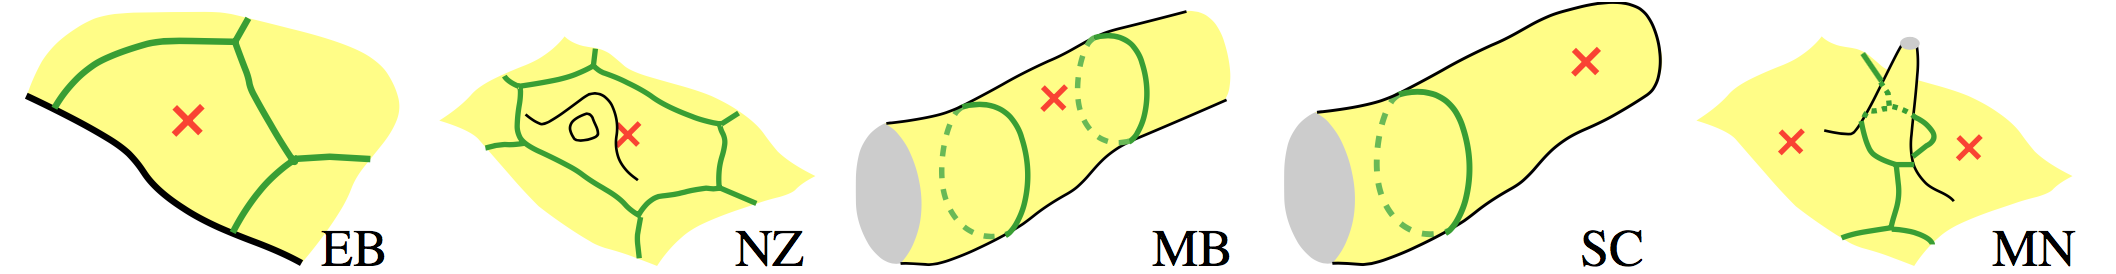
\includegraphics[scale=0.4]{VoronoiConditions}
\caption{Conditions that the Voronoi diagram has to respect in order to generate a 2-manifold triangulation \cite{Gus07}}
\label{fig:voronoi_conditions}
\end{figure}

In our case, some configurations cannot happen.
\textit{Nonzero genus} is not a possible cases, because by definition the depthmap represents the parameterization of the visible part of the scene. Thus the surface (or the multiple surface components) obtained after scanning have a zero genus and each Voronoi cell also, since each cell is a subset of the surface acquired.
\arnaud{There must be others that do not apply, but I can't really understand the \textit{Single curve tile boundaries} and \textit{Multiple neighbor instances} statements for now.}

Those conditions are verified after each Voronoi diagram computation. 

% \subsubsection{Power diagram from Gaussian curvature}
% Power diagrams are an extension of Voronoi diagrams to represent the fact that some sites can have a higher importance than others, for them to cover a larger area with respect to their neighbors. Similarly to what has been done for the poisson sampling in Sec.\ref{sec:poisson_sampling}, where the probability density function has been weighted by the absolute Gaussian curvature of the surface, it is possible to weight the influence of the Voronoi sites by the absolute Gaussian curvature, in order to create smaller cells (smaller weight) around the surface areas which have a high absolute curvature.

% \begin{equation}
% \label{eq:power_cell}
% 	V_S(v_i) = \{ x \in \mathbb{R}^n, \forall p \in S\, d(v_i,p) - w_i \leq d(v_j,p) - w_j\}
% \end{equation}

% \arnaud{Subsubsection incomplete : more explanation about the way to compute the weights (using the curvature values) in order for the Voronoi cells size to vary smoothly.}

\subsection{Lloyd relaxation}
Now that each valid pixel of the depthmap is included in a Voronoi cell, sites are going to be moved, in order for them to be more evenly spaced locally.

Each Voronoi cell can be in two different configurations : 
\begin{itemize}
	\item \textbf{the cell doesn't touch a border}. This means that no pixel being part of the Voronoi cell belongs to the border.
	In this configuration, the cell's site is moved to the centroid of its cell
	\item \textbf{the cell touches a border}. This means that at least one pixel being part of the Voronoi cell belongs to the border.
	In this configuration, the cell's site is moved to the orthogonal projection of the centroid of the cell on the border of the cell.
\end{itemize}

The centroid $z_i^*$ of the Voronoi cell $V_i$ can be obtained using the following integral :

\begin{equation}
		z_i^* = \begin{cases}
		Proj(\frac{\int_{V_S(v_i)} x\rho(x)\,dx}{\int_{V_S(v_i)} \rho(x)\,dx}) , & \text{if $|B_{V_i}| > 0$}, \\
		\frac{\int_{V_S(v_i)} x\rho(x)\,dx}{\int_{V_S(v_i)} \rho(x)\,dx}, & \text{otherwise}, 
		\end{cases}
\end{equation}

where $z^*$ is the centroid of the Voronoi cell $V_S(v_i)$ and $\rho(x)$ a probability density function defined over the domain $S$.
In our discrete case (where the domain is a depthmap), the integral can be re-written as the sum over all the pixels $p$ belonging to a Voronoi cell : 

\begin{equation}
		z_i^* = \begin{cases}
		Proj(\frac{\sum_{p_j \in V_S(v_i)} p_j\rho(p_j)}{\sum_{p_j \in V_S(v_i)} \rho(p_j)}) , & \text{if $|B_{V_i}| > 0$}, \\
		\frac{\sum_{p_j \in V_S(v_i)} p_j\rho(p_j)}{\sum_{p_j \in V_S(v_i)} \rho(p_j)}, & \text{otherwise}, 
		\end{cases}
\end{equation}

\section{Surface triangulation}
\label{sec:surface_triangulation}
Before triangulating, we need to define whether Voronoi cells belong to the same neighborhood (same surface area) or not. In comparison to the typical Delaunay dual-triangulation obtained from the Voronoi diagram, here we don't want to connect by an edge every pair of Voronoi cells having a common frontier in 2D. Some cells belong to different surface areas and then shouldn't be linked together.
For this we will use the borders that were constructed in \ref{sec:border_marking}.
We consider that two Voronoi cells $V_i$ and $V_j$ are belonging to the same neighborhood if there is no border separating them, meaning that there exists a non-empty set of non-border pixels belonging to $V_i$ which are neighbor (considering the 6-neighborhood we defined) to at least 1 pixel of the pixels belonging to $V_j$.

\begin{figure}[ht]
\centering
\scalebox{0.05}{
\begin{tikzpicture}[spy using outlines={circle,red,magnification=7.5,size=40cm, connect spies}]
\node {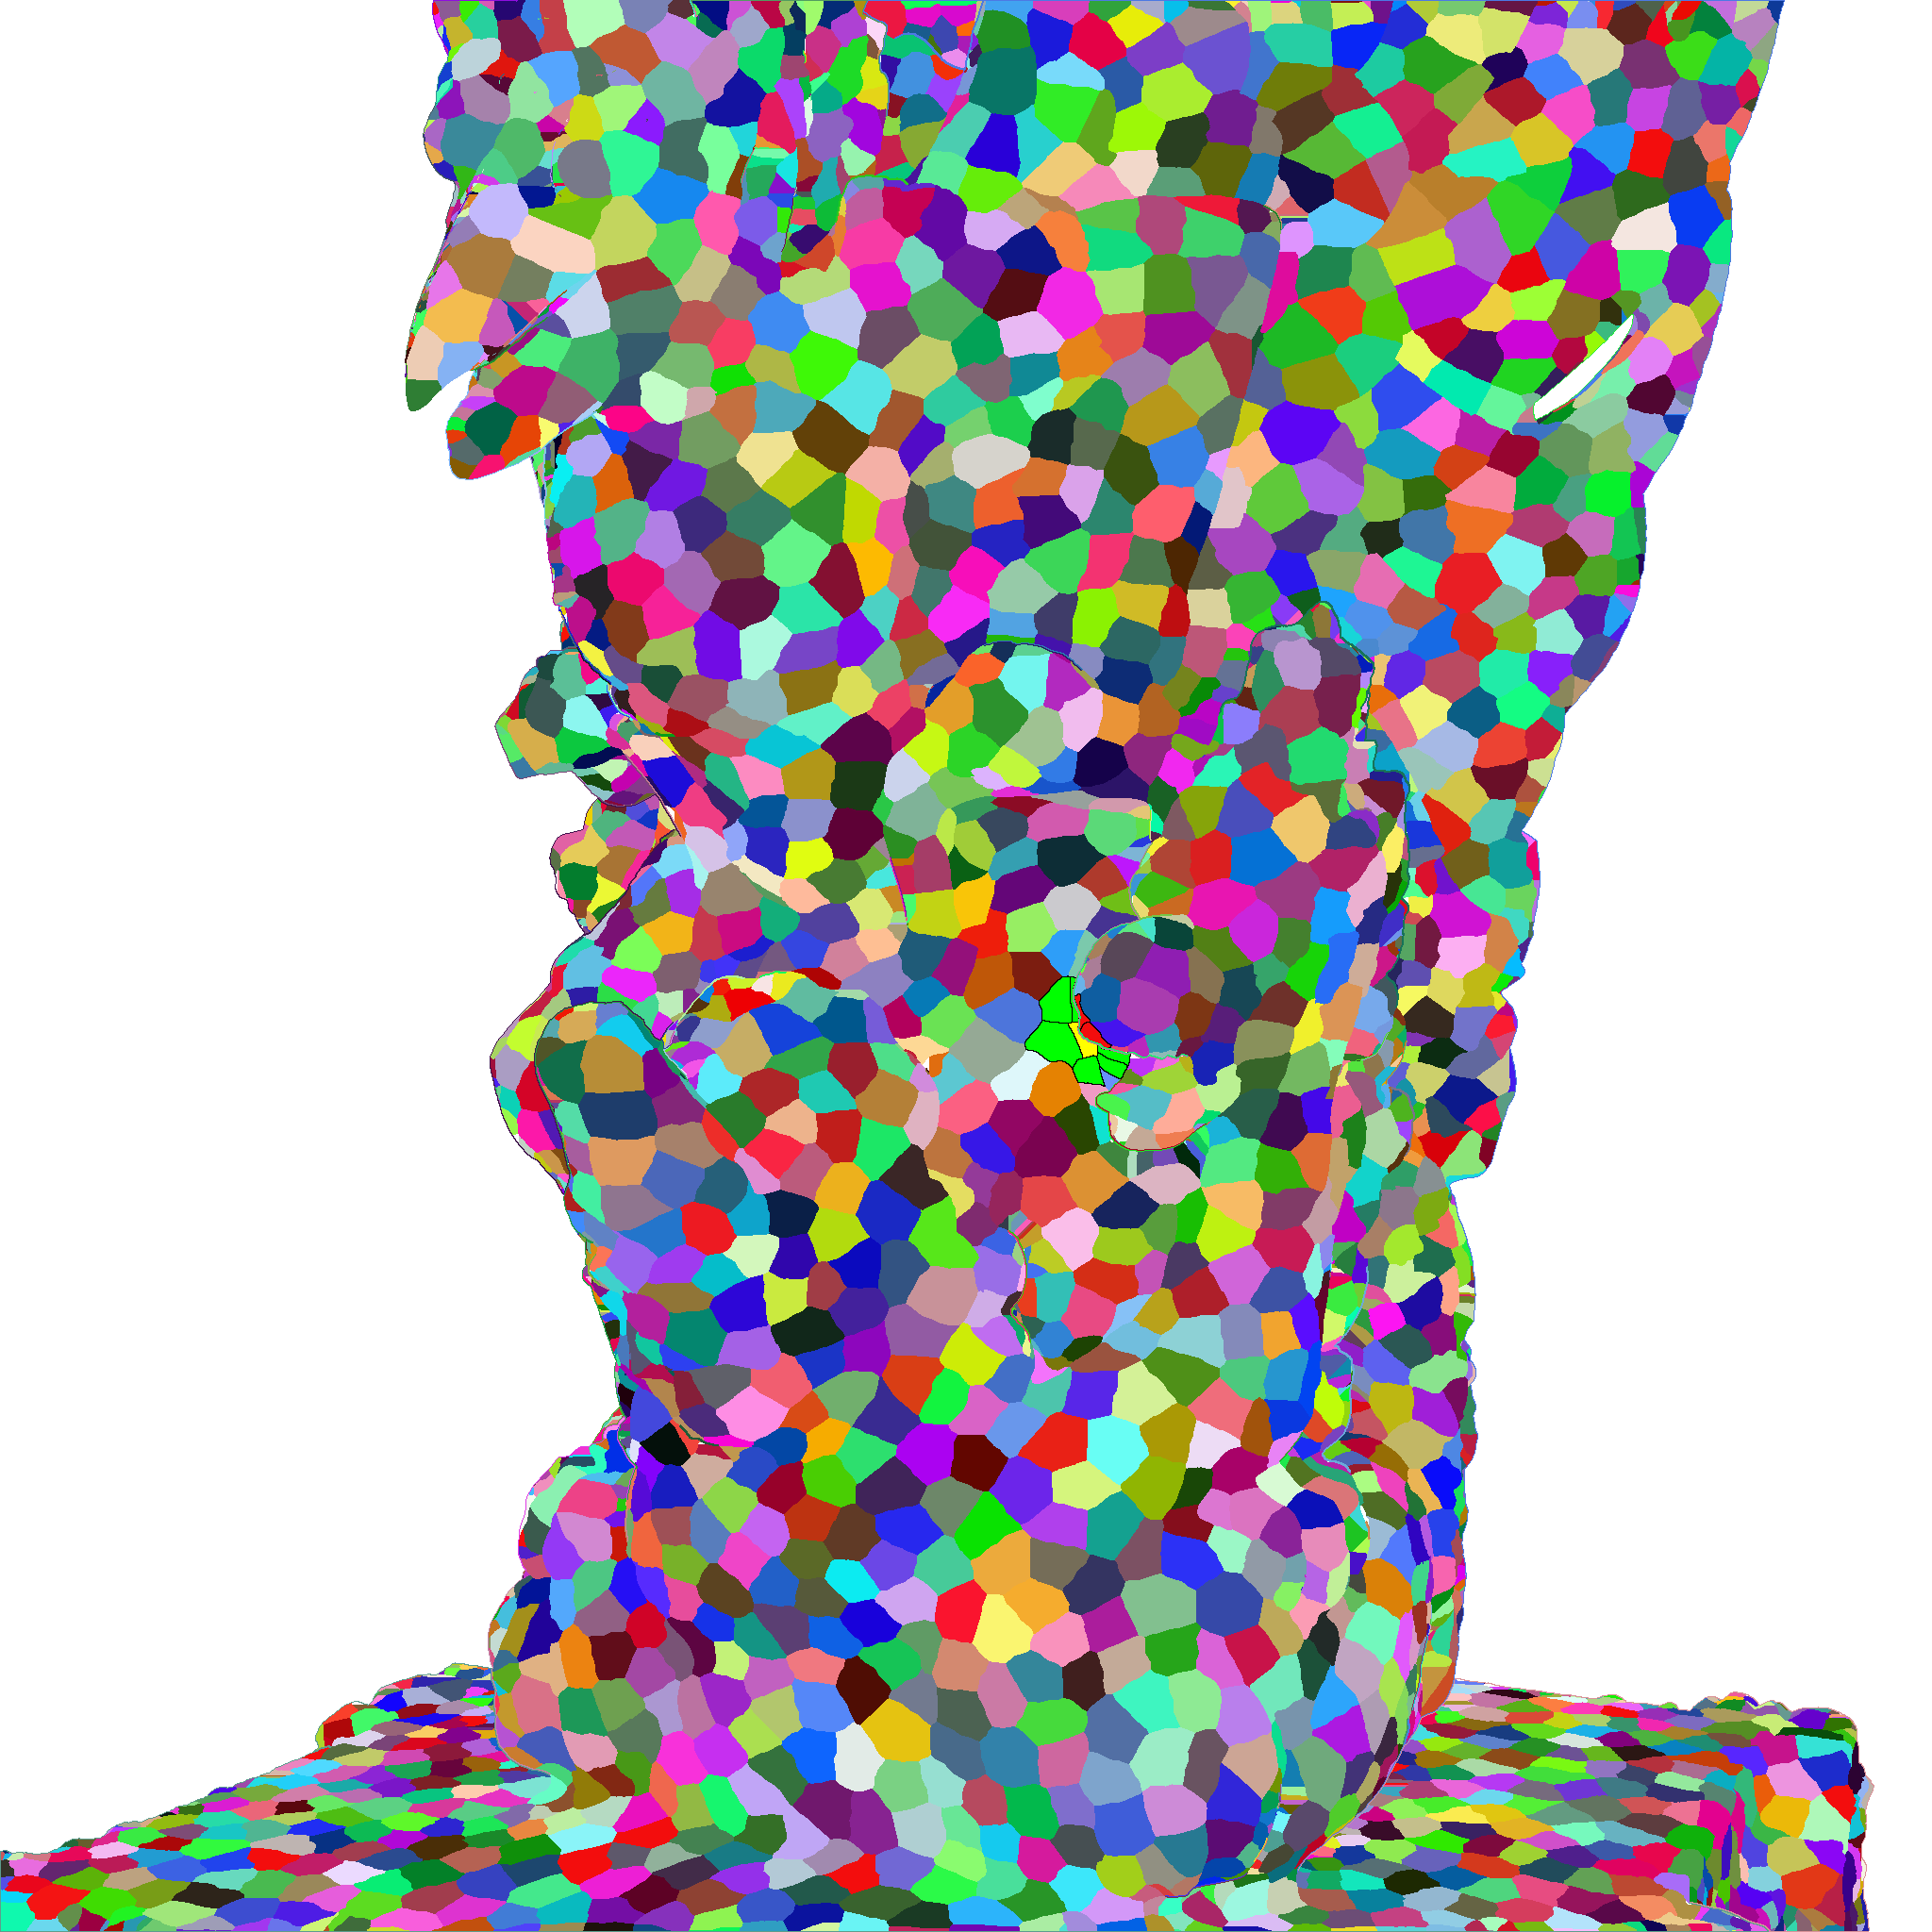
\includegraphics{Images/VoronoiDiagram3DBordersNeighborhood-Garuda}};
\spy on (4.25,-2.75) in node [left] at (100,-2.75);
\end{tikzpicture}
}
\caption{Neighborhood of a Voronoi cell (in yellow) $V$. In all the cells that have a common frontier with $V$, the cells colored in green belong to the neighborhood of the cell, whereas the ones colored in red don't.}
\label{fig:voronoi_cell_neighborhood}
\end{figure}

Considering the neighborhoods computed, we define our triangulation as being an altered dual representation of a Voronoi diagram, where edges are only connecting cells belonging to the same neighborhood (Figure \ref{fig:voronoi_diagram_triangulation}).
This allow to generate a triangulation where only points belonging to the same surface areas are triangulated together.

\begin{figure}[ht]
\centering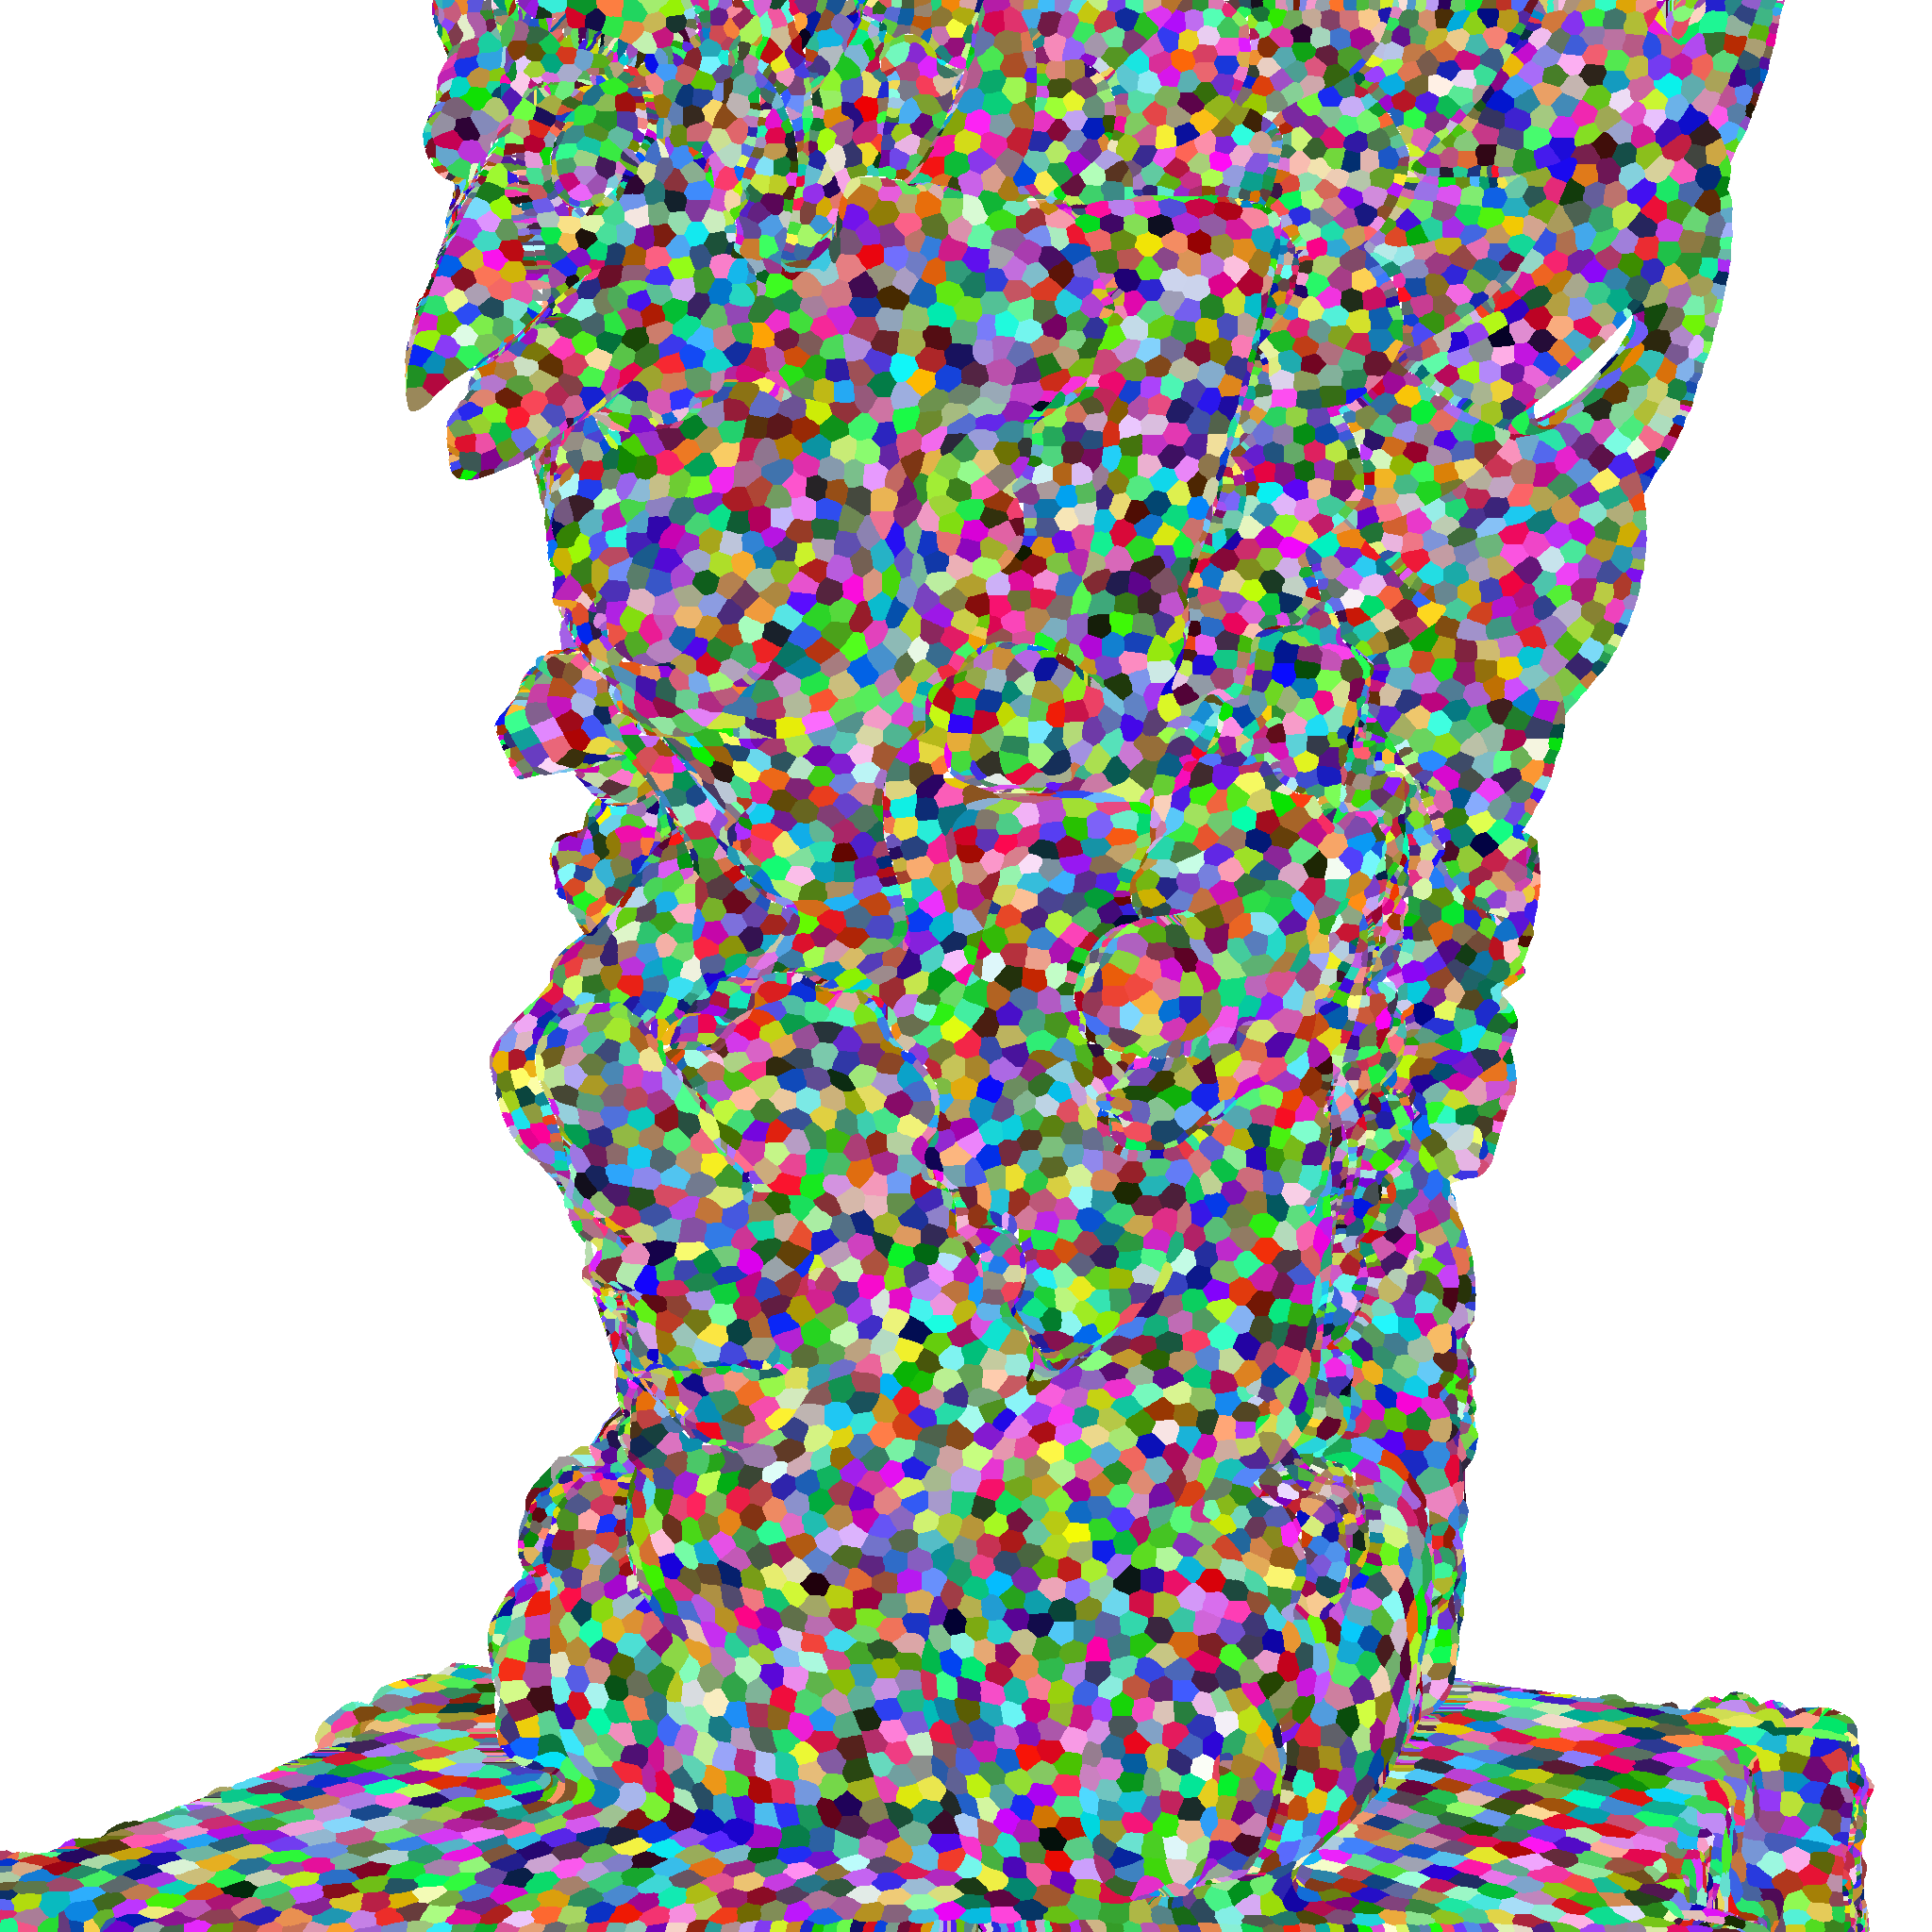
\includegraphics[scale=0.05]{VoronoiDiagram2D-Garuda}
\centering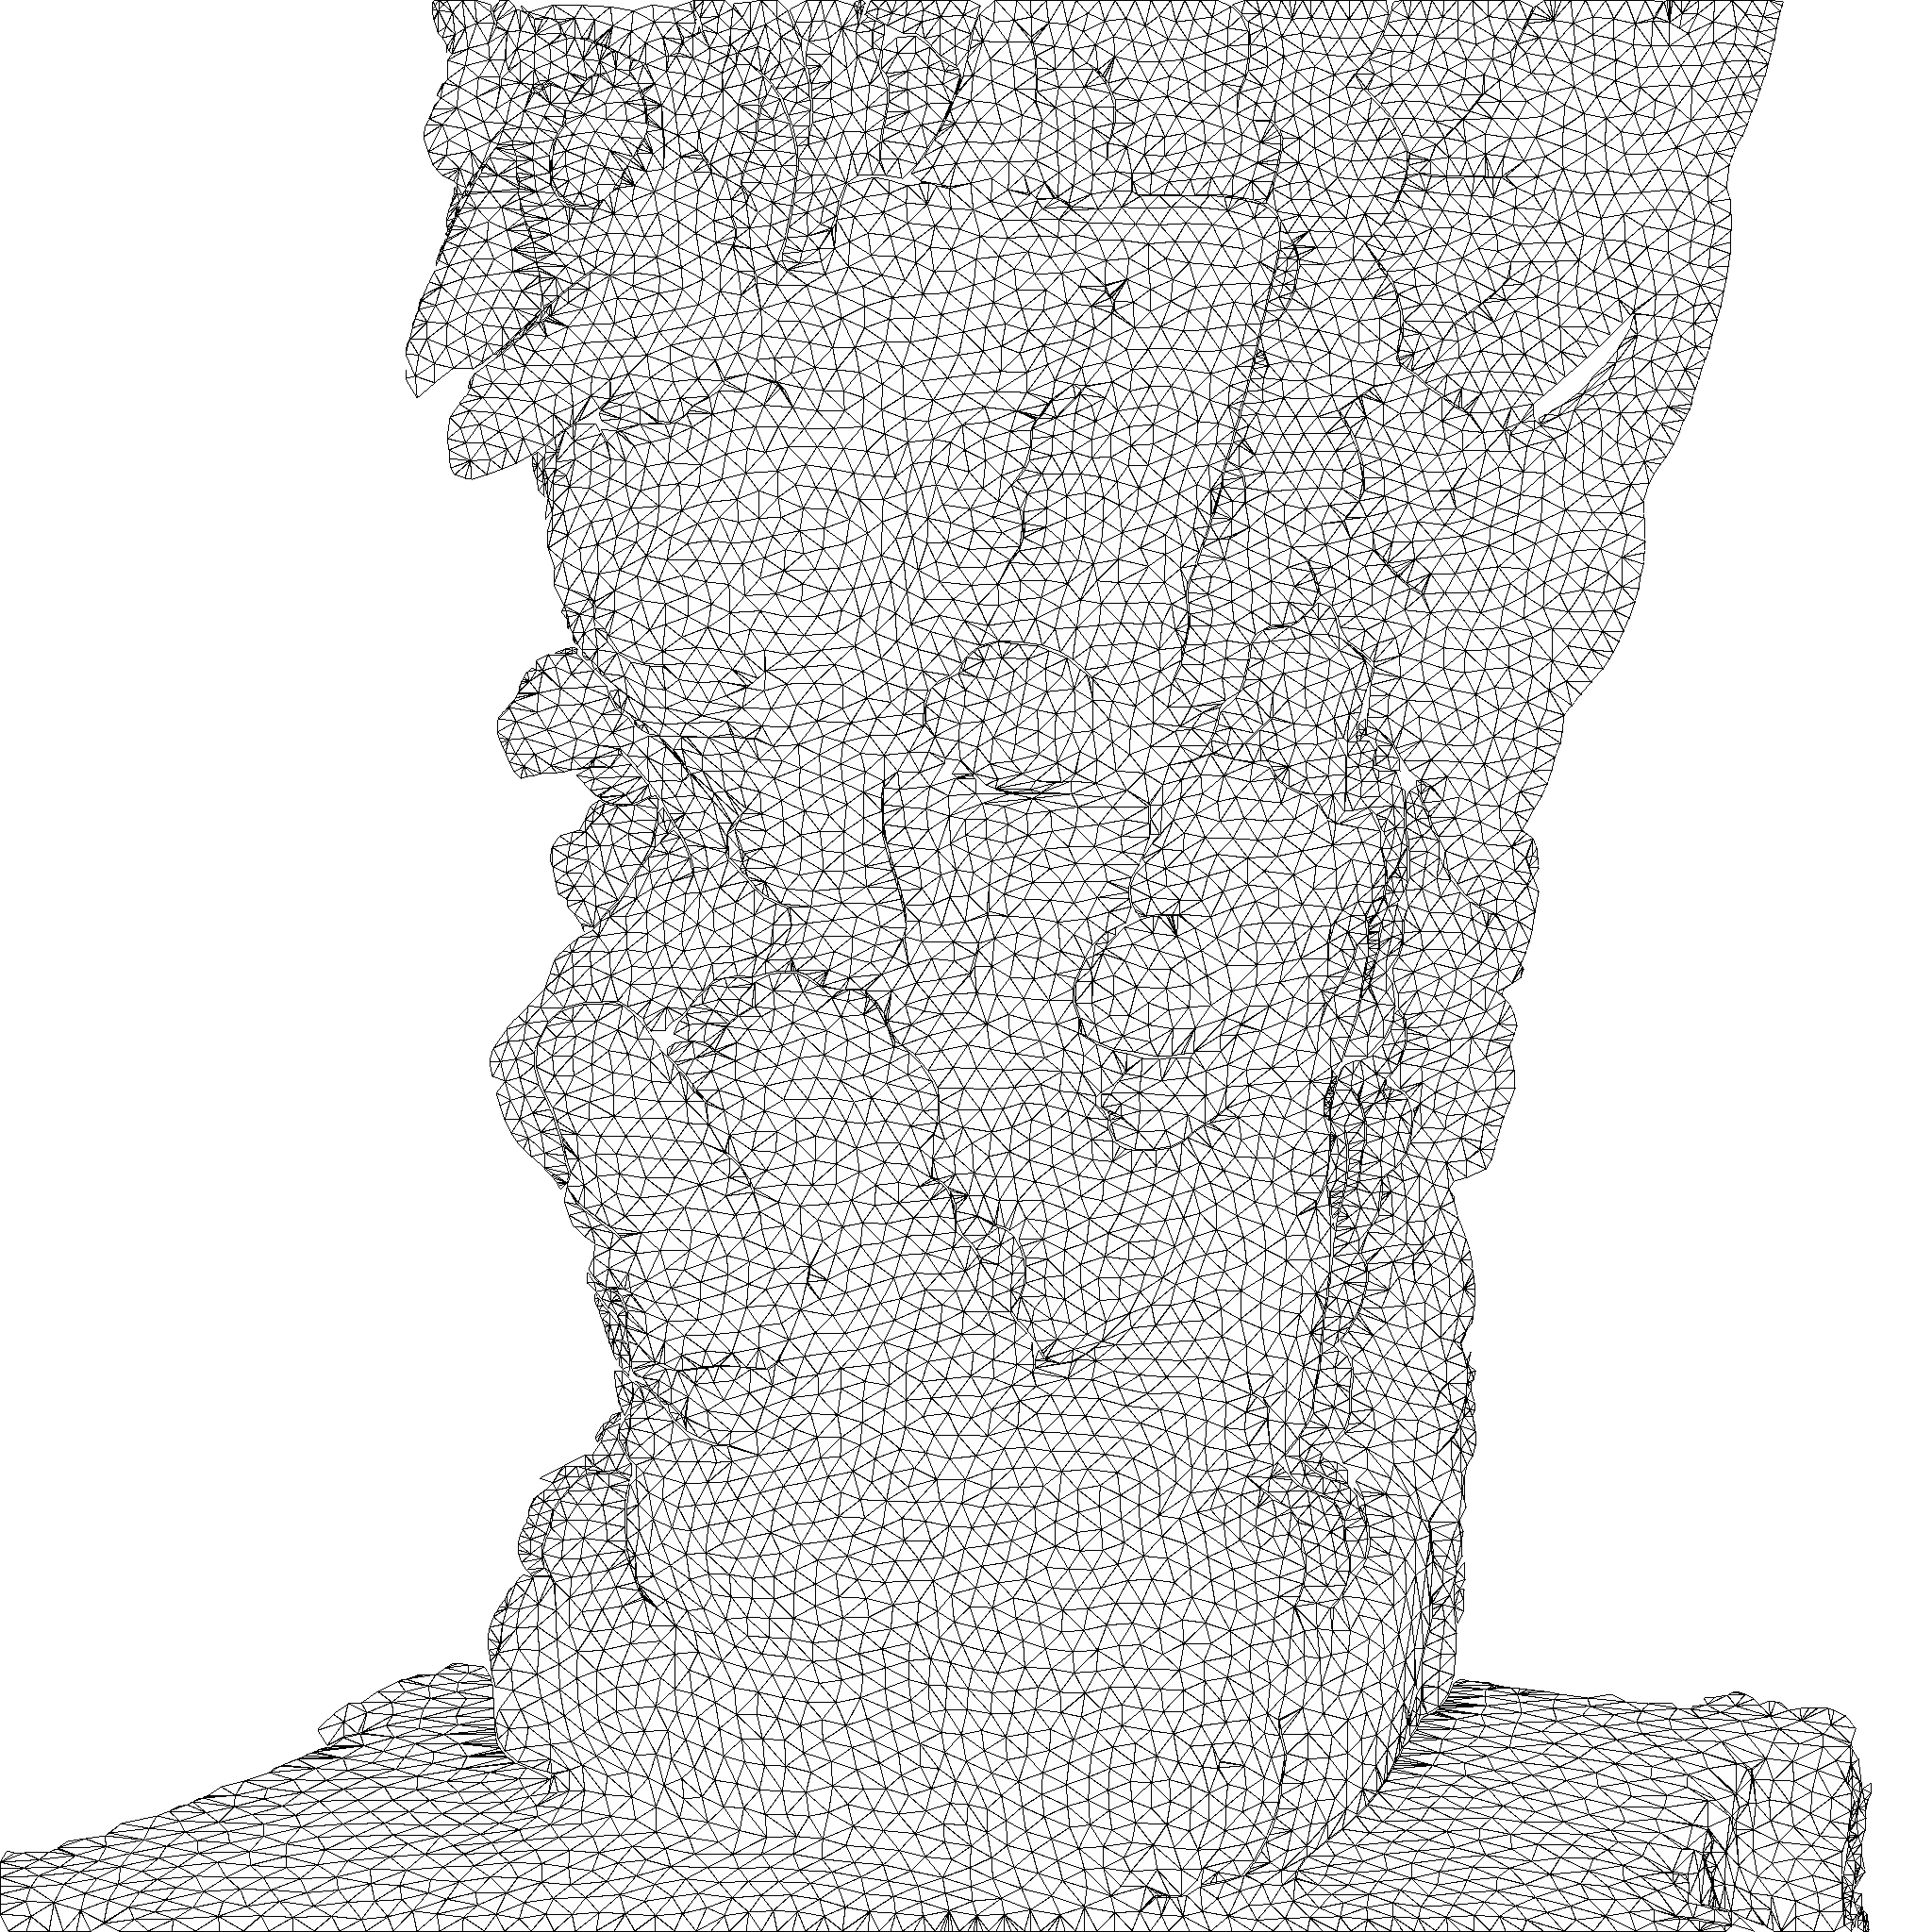
\includegraphics[scale=0.05]{Triangulation2D-Garuda}
\centering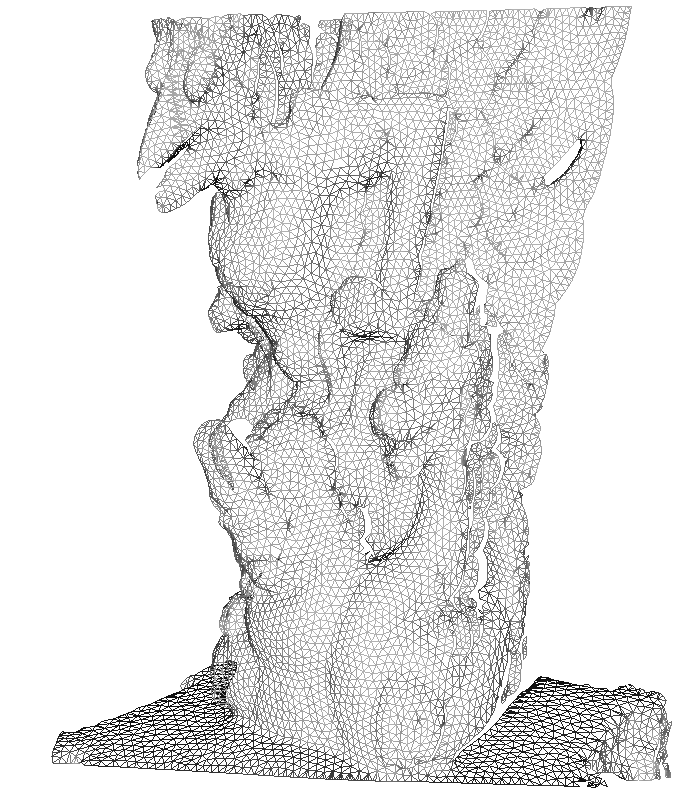
\includegraphics[scale=0.13]{Triangulation2DEmbedded-Garuda}
\caption{Voronoi diagram (a) and triangulation obtained as an altered dual representation of the Voronoi diagram (b).}
\label{fig:voronoi_diagram_triangulation}
\end{figure}

\section{Surface subdivision}
\label{sec:surface_subdivision}


%----------------------------------------------------------------------------------------
%	BIBLIOGRAPHY
%----------------------------------------------------------------------------------------
\bibliographystyle{alpha}
\bibliography{bibliography}

\printindex

\begin{appendices}
\section{Gaussian curvature}
\label{sec:gaussian_curvature}
The Gaussian curvature $K$ of a surface $S$ at a point $p$ is the product of the principal curvatures, $\kappa_1$ and $\kappa_2$ :

\begin{equation}
	K = \kappa_1\kappa_2
\end{equation}

Principal curvatures measure how much the surface bends in the two orthogonal directions where the surface bends the most.

The Gaussian curvature is an intrinsic measure of the curvature of a surface. 
As stated by Gauss in \cite{Gau28} through his \textit{theorema egregium}, the Gaussian curvature of an embedded smooth surface in $\mathbb{R}^3$ is invariant under local isometries.
This means that no matter how the surface is bent, its total Gaussian curvature remains the same, and is related to the Euler characteristic, based on the topology of the surface.

\subsection{Gaussian curvature approximation}
In \cite{MMPB02}, an approximation of Gaussian curvature is given by using the vertex angular deficit expression :

\begin{equation}
	K(v_i) = \frac{2\pi -\sum_{v_j \in \mathcal{N}_1(v_i)} \theta_{ij}}{\mathcal{A}_{mixed}},
\end{equation}

where $\mathcal{N}_1$ represents the 1-ring neighborhood of $v_i$, $\theta_{ij}$ is the angle of $v_jv_iv_{j-1}$ at $v_i$ which is given by the following formula : 

\begin{equation}
	\theta_{ij} = \arccos(\frac{\overrightarrow{v_iv_j} \cdot \overrightarrow{v_i v_{j-1}}}
	{\norm{\overrightarrow{v_iv_j}}^2\norm{\overrightarrow{v_iv_{j-1}}}^2}),
\end{equation} 

and $\mathcal{A}_{mixed}$ represents the surface area around the vertex $v_i$ : 

\begin{algorithm}
\caption{$\mathcal{A}_{mixed}$ computation}
\begin{algorithmic}
\State $\mathcal{A}_{mixed}$ = 0
\ForAll{triangle $T$ from the 1-ring neighborhood of x}
	\If{T is non-obtuse}	//Voronoi area can be considered
		\State $\mathcal{A}_{mixed} \mathrel{+}= \frac{1}{8} \sum\limits_{v_j \in N_1(v_i)} (\cot \alpha_{ij} + \cot \beta_{ij}) \norm{v_i-v_j}^2$
	\Else
		\If{the angle of $T$ at $x$ is obtuse}
			\State $\mathcal{A}_{mixed} \mathrel{+}= area(T)/2$
		\Else
			\State $\mathcal{A}_{mixed} \mathrel{+}= area(T)/4$
		\EndIf
	\EndIf
\EndFor
\end{algorithmic}
\end{algorithm}

\arnaud{ADD FIGURE GAUSSIAN CURVATURE}

\section{Proofs}

\begin{equation}
	y_i = \frac{\int_{V_i}xf(x)dx}{\int_{V_i}f(x)dx},
\end{equation}

where : 

\begin{equation}
	f(x) = 
    \begin{cases}
      \frac{1-\varepsilon}{|B_{V_i}||C|}, & \text{if}\ x \in B_{V_i} \\
      \frac{\varepsilon}{(|V_i|-|B_{V_i}|)|C|}, & \text{if}\ x \not\in B_{V_i}
    \end{cases}
\end{equation}

\begin{equation}
	\sum_{i=1}^k \int_{V_i}f(x)dx = 1
\end{equation}

\begin{align*}
	\sum_{i=1}^k \int_{V_i}f(x)dx 
	&= \sum_{i=1}^k \int_{V_i \setminus B_{V_i}}\frac{\varepsilon}{(|V_i|-|B_{V_i}|)|C|}dx + \int_{B_{V_i}}\frac{1-\varepsilon}{|B_{V_i}||C|}dx \\
	&= \sum_{i=1}^k \frac{\varepsilon}{(|V_i|-|B_{V_i}|)|C|}\int_{V_i \setminus B_{V_i}}dx + \frac{1-\varepsilon}{|B_{V_i}||C|}\int_{B_{V_i}}dx \\
	&= \frac{1}{|C|} \sum_{i=1}^k \frac{\varepsilon}{|V_i|-|B_{V_i}|}\int_{V_i \setminus B_{V_i}}dx + \frac{1-\varepsilon}{|B_{V_i}|}\int_{B_{V_i}}dx \\
	&= \frac{1}{|C|} \sum_{i=1}^k \varepsilon + 1 - \varepsilon\\
	&= \frac{k}{|C|} = 1
\end{align*}

\end{appendices}

%----------------------------------------------------------------------------------------

\end{document}
